
\documentclass[12pt,a4paper]{article}
% \usepackage[english]{babel}
% \usepackage[utf8x]{inputenc}
\usepackage{tocbibind}

\usepackage{array}
\usepackage{longtable}
\usepackage{graphicx} % Required for inserting images.
\usepackage{float}
\usepackage[margin=2cm]{geometry}
\parskip 4.2pt  % Sets spacing between paragraphs.
% \renewcommand{\baselinestretch}{1.5}  % Uncomment for 1.5 spacing between lines.
\parindent 8.4pt  % Sets leading space for paragraphs.
\usepackage[font=sf]{caption} % Changes font of captions.
\usepackage[margin=2cm]{geometry} % Sets the left and right margins to 2cm.
\usepackage{listings}
\lstdefinelanguage{alloy}{
  keywords={sig,abstract,extends,check,pred,fact,assert,run},
  keywordstyle=\color{blue}\bfseries,
  sensitive=true,
  comment=[l]{--},
  commentstyle=\color{green}\ttfamily,
  %stringstyle=\color{red}\ttfamily
}
\geometry{
  top=2.5cm,    % Adjust the top margin here
  bottom=2.5cm, % Adjust the bottom margin here
}
\usepackage{amsmath}
\usepackage{amsfonts}
\usepackage{amssymb}
\usepackage{siunitx}
\usepackage{verbatim}
\usepackage{afterpage}
%\usepackage{hyperref} % Required for inserting clickable links.
%\usepackage{natbib} % Required for APA-style citations.
\usepackage{makeidx} % Required for creating the index
\usepackage{enumitem}

\includeonly{
	1Introduction/1Introduction_layout,
	2Overall_Description/2Overall_Description_layout,
	3Specific_Requirements/3Specific_Requirements_layout,
	4Alloy/4Alloy_layout
}
\graphicspath{
	{1Introduction/res/}
	{2Overall_Description/res/}
	{3Specific_Requirements/res/}
	{3Specific_Requirements/res/SD/}
	{4Alloy/res/}
	}
	
\newcommand{\app}{CodeKataBattle }



\renewcommand{\rmdefault}{ptm} % Times font

\begin{document}
\begin{titlepage}
    \centering
    
\includegraphics[width=6.5cm]{Logo_Politecnico_Milano.png} \par
    \vspace*{2.3cm}
    {\LARGE Requirement Analysis and Specification Document}\par
   
   
    \vspace*{0.8cm}
    {\Large \textbf{CodeKataBattle}}\par
    \vspace*{6.8cm}
    
    \setlength{\tabcolsep}{1.1cm}
    \large Authors \par
    \begin{table}[h]
      \centering
      
      \renewcommand{\arraystretch}{2} 
      \begin{tabular}{c c c }
        \textbf{Name} & \textbf{Surname} & \textbf{ID} \\
        \hline
        Alessandro & Saccone & 11013852 \\
        
        Matteo & Sissa & 10972783  \\
        
        Sara & Zappia & 11016799\\
        
      \end{tabular}
    \end{table}
    \vspace*{1.3cm}
    \small{ Version 1.0 - 22/12/2023}\par
    \vspace*{0.3cm}
    \small{ A.Y. 2023/2024}\par
\end{titlepage}

\clearpage
\tableofcontents
\clearpage


\newcommand{\sourcepath}{1Introduction/src/}

\section{Introduction}
\input{\sourcepath 1.1Purpose}
\input{\sourcepath 1.2Scope}
\subsection{Definitions, Acronyms, Abbreviations}
\input{\sourcepath 1.3.1Definitions}
\input{\sourcepath 1.3.2Acronyms}
\input{\sourcepath 1.3.3Abbreviations}
\input{\sourcepath 1.4RevisionHistory}
\input{\sourcepath 1.5ReferenceDocuments}
\input{\sourcepath 1.6DocumentStucture}
\newpage

\clearpage
\section{Overall Description}
\subsection{Product Perspective}
\subsubsection{Scenarios}
\textbf{SCENARIO 1 - Educator logs in the system} \\
    Emanuele is a professor at Politecnico di Milano in the Computer Science department. He has just discovered a new application called \app that allows educators to organize tournaments of students to make them compete on coding battles.\\
    Emanuele is very enthusiast about the idea because he thinks it might be a great opportunity for his students to better their software development and problem solving skills. He therefore opens \app on his laptop. The first interface showing up is the log in interface, in which the application asks Emanuele to sign in using his GitHub personal account. He clicks on the button to be redirected to the GitHub authentication page and uses his credentials as required. GitHub calls back the \app platform and now Emanuele is logged in and can start experimenting with this brand new system.\\
    
    \textbf{SCENARIO 2 - Student logs in the system} \\
    Matteo is a student enrolled in a Computer Science master's degree at the University of Barcelona. He's passionate about coding and software development in general. One day, he comes across a new app called \app that allows students to compete against each other in coding battles organized by educators from many universities spread across the world.  \\
    This application immediately catches his attention, so he decides to open it on his laptop. The first interface showing up is the log in interface, in which the \app platform asks Matteo to sign in with his personal GitHub account. Matteo clicks on the button that redirects to the GitHub authentication page and logs in as requested.
    Now, he's signed in the platform and can start playing around with it to see if he likes it.\\
    
    \textbf{SCENARIO 3 - Educator creates a new tournament}\\
    Mario is a renowned university professor in the field of Software Engineering. He has been using the \app application for a while now, but he's never organized a tournament on this platform.
    One day, he decides to create his first tournament on \app. So, he opens the application and signs in. Among the various buttons that are available on the educators' home page of the platform, he clicks on the one to create a new tournament. As a consequence, \app opens up a window in which various parameters can be set for the new tournament. Mario can set the name of the tournament, a description of it and the registration deadline by which students are asked to subscribe to the tournament if interested. Moreover, there is a section dedicated to the definition of badges (rewards) to be assigned to students at the end of the tournament based on some goals or achievements. Mario can declare on \app what kind of rewards he wants allocate and for each reward the achievement(s) that have to be accomplished by a student in order to earn the badge.\\
    After filling in the all fields of the form, Mario can confirm the creation of the tournament and the application will show him the newly-created tournament page.
    \app will also send a notification to all the student on the platform informing them of the new available tournament.\\

    \textbf{SCENARIO 4 - Educator creates a new battle}\\
    Alex is a professor at the University of London specialized in artificial intelligence. Lately, he's been using the \app platform to help his students practice on some algorithms that he's explaining during the lectures. One morning, he comes up with a new idea for a code kata battle that may be very beneficial for the students that are going to take his exam in the following months. Thus, he seats at the desk in his bedroom and starts writing a textual description of the battle, along with the build automation scripts and test cases that are required by \app in order to build and test the students' solutions to the exercise. Once done with these tasks, Alex takes his laptop and opens the \app application. He logs in through his GitHub account and clicks from the home page the button to create a new battle. A new interface pops up displaying all the tournaments in which Alex has permissions to publish battles (so the tournaments Alex created and the ones other educators granted Alex permissions on). Alex selects one of these tournaments and the form to set the battle's parameters and characteristics shows up. Through this interface, Alex is able to upload the textual description, build automation scripts and test cases that he previously designed; he also set the battle's name, the registration and submission deadlines, the minimum and maximum number of students per team allowed. Moreover, the aspects on which \app has to base its automatic evaluations of the students' solutions (reliability, maintainability...) can be defined and it is possible to establish whether to require a consolidation stage at the end of the battle (in order to allow Alex to assign personal scores).
    Once all of these parameters have been set, Alex clicks on the confirmation button and the page dedicated to the newly created battle pops up on his display.
    Immediately after this, \app will fire a notification message to all the students subscribed to Alex's tournament in order to inform them of the new available battle.\\

	\textbf{SCENARIO 5 - Educator grants the permission to publish battles in his/her tournament to another educator}\\
	George is a professor at MIT's Software Engineering department. Lately, he's been actively using the \app software because he initiated a tournament of coding challenges for students centered around the Python programming language. He's published many battles over the last week, and that's why he's running out of ideas for new problems to propose. That's why he decides to ask for some help from one of his closest colleagues, Laura. In order to allow Laura to publish battles inside George's tournament, George has to grant her permissions to do so. Thus, George opens the \app application and clicks on the button to display the tournaments he created. Among these, he selects the one in which he wants Laura to help him. The home page of the selected tournament pops up and there is a button to grant publishing permissions to another educator. Once clicked, George is able to search for Laura's account through her username on the platform and then send her a request to be added as an educator with publishing permissions inside his tournament. Once these steps have been carried out, Laura is able to see George's request on her profile and accept it. George's tournament will then appear in the list of tournaments in which she can create battles. Now George will no longer be the only one keeping the tournament alive with new battles.\\

    \textbf{SCENARIO 6 - Student subscribes to a tournament}\\
    Alessandro is an artificial intelligence student at the Technical University of Munich. It has been a while since the last time he coded a program of any kind, so he feels a little bit rusty on that. He would like to brush up on this skill and he decides to use the new app \app for this purpose.
    After logging in the system, \app displays all the available tournaments on the platform. Thus, Alessandro starts browsing this list, searching for something that he might find interesting. 
    At some point, he stumbles upon a tournament created by one of his favorite professors at his university, so he clicks on it and the home page of the tournament pops up. George clicks on the button to subscribe and confirms his choice. Consequently, \app moves the selected tournament in the list of tournaments Alessandro is subscribed to.
    From this moment on, Alessandro will be notified by the \app app every time a new battle will be published inside the tournament.\\

    \textbf{SCENARIO 7- Student joins a battle on his/her own (without a team)}\\
    Lorenzo is a student at the University of Pisa specialized in data management. He's been eagerly trying to reach the first position in a tournament of the \app application, but he's still some points behind the first in the ranking. He doesn't want to give up, so he opens \app and navigates to the tournament in which he's competing. In order to get additional points he has to join another battle. So he commences the search for the battle, reading some descriptions of the battles published in the tournament whose registration deadline hasn't passed yet. He eventually finds one that might be suitable for him, so he clicks on the button to join it. \app promptly shows Lorenzo the description page of the battle, where there's a button to join it. Once clicked, an interface pops up in which it is possible to select whether to join the battle as a single player or with other students in a team. Since Lorenzo usually prefers to work on his own, he opts for the single player and confirms.
    The battle is therefore added to the list of battles Lorenzo is participating in. Lorenzo will be able to submit his code solutions when the registration deadline passes and \app will have created the GitHub repository dedicated to the battle.\\

    \textbf{SCENARIO 8 - Student joins a battle with other students as a team}\\
    Lucia is a student at the Politecnico di Torino university and she's enrolled in the cybersecurity program. Her group of university friends have been talking incessantly about creating a team on the new \app application to solve together a coding battle proposed by one of their professor specialized in cryptography called Adrian. She lets her friends persuade her to do that, so she opens the \app application on her laptop and navigates to the tournament that contains the interesting battle. She and her friends are already subscribed to such tournament, since it is a very popular one organized inside the university, therefore she doesn't have to sign up for that. Then, Lucia spots the coding challenge her friends were talking about and clicks on it. Since the registration deadline hasn't passed yet, \app promptly shows the interface to join the battle, in which it is possible to select whether to sign up as a single player or with other students as a team. Obviously she picks the latter option and a new window pops up, in which Lucia has the possibility to search by username her friends on the platform and send them a request to join the battle in her team. Once this process is carried out, Lucia confirms and the \app application displays the entry page of the battle. The battle is therefore added to the list of battles Lucia is participating in.
    Lucia's friends will be able to take part in the battle as soon as they accept the request sent by the system. At that point, the battle will also be added by \app to the list of battles in which they are competing.
    Lucia and her friends will be able to submit their code solutions as soon as the registration deadline for the battle passes and \app creates the dedicated GitHub repository.\\
    
    \textbf{SCENARIO 9 - Student receives the link of the GitHub repository dedicated to a battle and starts pushing his code solutions on the forked branch of the GitHub repository}\\
    Francesco is a student at the University of Edinburgh where he studies computer engineering. A couple of days ago he joined a new battle on the \app application which was very appealing to him as it was about optimization algorithms. He has been very busy with some commitments that he had taken, so he hasn't opened \app since the subscription to the battle. Luckily, at around midday, he receives a notification from the app saying that the battle was open (since the registration deadline had passed) and that it was possible to hand in the code solutions to the challenge on a forked branch of the dedicated GitHub repository. The link to the GitHub repository was also attached to the notification message.
    This alert from \app suddenly reminds Francesco of the battle. So he runs back home from the university and first of all sets up the GitHub environment. He forks the main branch of the GitHub repository dedicated to the battle and also writes an automated GitHub workflow with GitHub Actions in order to fire a notification from GitHub to the \app platform every time he pushes a new code solution to the forked branch.
    At this point, Francesco is able to start pushing his solutions to the forked branch on GitHub and see the corresponding scores on \app. So he writes a code block that might pass the test cases of the battle and submits it on his GitHub branch.\\
    GitHub will immediately fire a notification to the \app platform. As a consequence, \app downloads Francesco's code solution and uses the build automation scripts provided by the educator that published the battle in order to build the code. At this point, if \app is not even able to build the code solution, an error message is returned to Francesco stating the problem. In the other situation, the test cases (provided by the educator that created the battle) are employed to verify the correctness of the solution. Moreover, \app exploits some external static analysis tool to rate some other parameters of the solution (chosen by the educator that created the battle) like security, maintainability and so on. These pieces of information are put together with the time passed since the beginning of the battle in order to assign a score to Francesco's solution.
    In a few moments after the submission of the solution, Francesco notices on the \app platform the score assigned to his solution and also his updated position in the battle ranking, based on the new score.\\
  
    \textbf{SCENARIO 10 - Educator manually evaluates the students' code solutions of one of his/her battles during the consolidation stage}\\
    Michele is a meticulous computer science teacher in a little high school in Rome. Lately, he's been publishing several battles on the \app platform for his students to let them exercise on some new algorithms he explained during the lectures. Since he wants to personally assess the code that his students write, he always specifies at battle creation time that a consolidation stage is required for his battles. Today, Michele knows that the submission deadline of one of his battles will pass at 6pm, and that after that time, the \app will allow him to assign a personal evaluation to his students' solutions. At 6:30pm, when Michele comes home from work, he makes himself a cup of tea and opens the \app platform. In the list of battles that he created, he clicks on the one that requires the consolidation stage to be carried out. A new interface shows up, where the list of teams subscribed to the battle is shown and for each team there is a field on the side where it is possible to type in the score Michele wants to assign. Within this interface, there is also a timer that specifies how much time Michele has to assess the code solutions. After the timer goes off, if Michele hasn't provided a score for each team in the battle, the consolidation stage won't be taken into account by \app in order to compute the final ranking of the battle.
    All the source code for the solutions is available for Michele on the GitHub platform, so he can review it all and complete the consolidation stage for the battle by the specified time frame.
    When the timer goes off, \app is able to draw the final ranking of teams for the battle and publish it on the platform. \app will also send a notification to all the participants of the battle to notify them of the available hierarchy of teams.\\

	\textbf{SCENARIO 11 - A battle terminates and the ranking of teams is published}\\
	Clara, a data analytics student enrolled in a Master's program at ETH Zurich university is impatiently waiting for the end of a battle on the \app platform. She's worked really hard over the last weekend in order to reach the first position in the ranking with a solution that scored 95/100. At 1pm, the submission deadline for the battle has finally passed. Since no consolidation stage was required by the professor who published the battle, \app immediately calculates the total ranking of teams and fires a notification to all the students participating in the battle. Also Clara receives the alert stating that the battle was over and that the final ranking was available on the app. She enthusiastically opens \app on her laptop just to find out that during the last 10 minutes before the submission deadline, another competitor handed in a solution that received a score higher than hers.\\ 

	\textbf{SCENARIO 12 - Educator closes a tournament that s/he previously created}\\
    Olivia is a famous professor in the field of Bioinformatics. Over a month ago, she decided to create a new tournament on the \app platform in which she's been started publishing coding battles that are biology-themed. Many students from all over the city in which Olivia lives liked the idea of this tournament and decided to take part in it. Now, since the tournament has been going on for over a month, the challenges are becoming more and more repetitive, therefore Olivia decides to officially close it. She opens the \app application on her laptop and logs in. In the home page, she clicks on a button to display the list of tournaments that she created. She selects the tournament she wants to close, clicks the button to close the tournament and confirms her choice. The \app platform immediately sends a notification to all the students subscribed to the tournament informing them that the tournament is now closed and the final ranking of students is available. Since \app always maintains updated the ranking of students in a tournament, there is no need to recalculate the ranking here, just to display it. Moreover, since Olivia defined some badges at tournament creation time, \app evaluates the sets of students that are eligible to receive these badges and assigns them accordingly. The personal profile of students that received a reward from the tournament is automatically updated by the app.\\

    \textbf{SCENARIO 13 - User opens the ranking of a tournament on the \app platform}\\
    Christian is a student at Princeton University where he specializes in game design and development. He knows that some of his classmates are participating in a tournament on the \app platform organized by some of the professor of the engineering department and he's very curious about the ranking of this tournament. So, he opens \app, logs in with his personal GitHub account and in the home page that is displayed right after the log in he can see all the tournaments available on \app. He scrolls a little bit down and eventually finds the tournament he was looking for. So he clicks on it and in the dedicated page, the total ranking of students is shown, updated with the very last scores assigned to the students' solutions. Christian can finally see how his classmates are positioned.\\

    \textbf{SCENARIO 14 - User opens the ranking of a battle s/he is involved in}\\
     Emily is a web development student at the University of Toronto. She's been working with her team on the solution for a battle on the \app platform for a while now, but she cannot get a score higher than 55/100. Since she doesn't know if that is going to be enough to reach the top 10 positions of the battle ranking, she decides to give a look at the partial ranking for the competition, to have an idea of how well the other teams are doing so far. So she opens the \app app on her laptop and navigates to the list of tournaments she's subscribed to. Once she's selected the correct tournament, she can see the list of battles belonging to that tournament that she signed up for and among them she picks the one she wants to see the ranking of. Consequently, \app checks whether Emily is actually involved in the battle or not and displays the ranking only in the affirmative case. 
     At the end, Emily discovers that she and her team are in the very last position!\\

    \textbf{SCENARIO 15 - User searches by username the personal profile of another user on the platform and looks at his/her badges}\\
    Filippo, a student at the University of Bologna, where he's conducting some important research on Cloud Computing, has been using the \app application to compete with other classmates on coding challenges. Since he's very competitive, he wants to give a look at his friends' profiles on the platform to check if they have obtained more badges than him. So he opens the \app application on his laptop, logs in and clicks on the search box in the home page to type in the username of one of his friends. Once he finds the correct user on the application, he clicks on it and \app displays the personal profile of this user. Filippo is able now to inspect the set of badges earned by his friend and compare them with the ones he obtained so far.\\
\clearpage

\subsubsection{Domain Class Diagrams}

The following class diagram provides a high-level view of the domain of interest for the \app platform. It is possible to notice elements that are external to the system (GitHub repositories, Users, Students, Educators) as well as the most meaningful internal ones (Tournaments, Battles, Scores, Rankings, Badges...). 
This diagram pursues the objective of showing the multiplicity relations between all of these components, along with the most relevant pieces of information (attributes) that characterize them.
As a remark to understand some of the multiplicity relations stated in the class diagram, only GitHub users that have already accessed \app once are considered, thus the 1:1 relationship between GitHubUser and User. Besides, the set of external GitHub repositories is restricted to those associated to a battle and the ones forked by the students from there.
\begin{center}
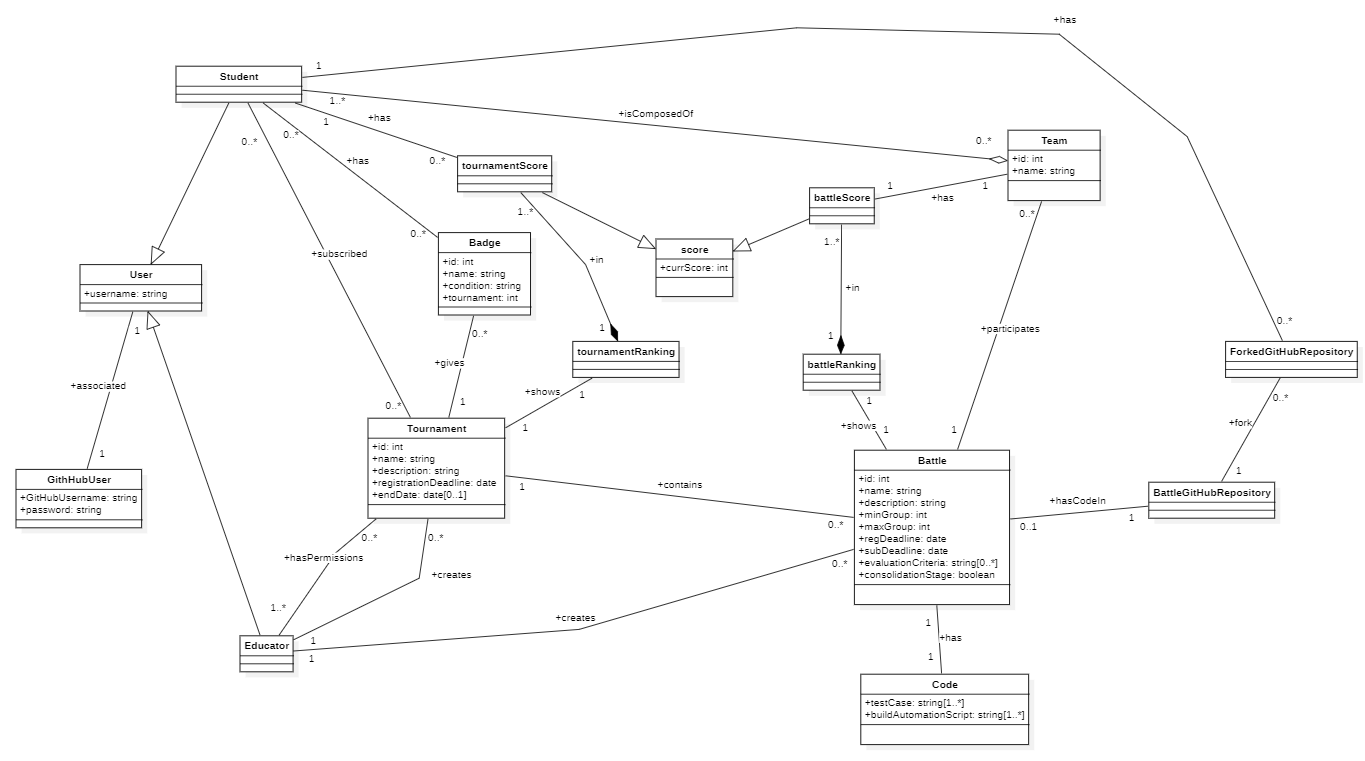
\includegraphics[angle=90,width=0.6\linewidth, scale=1.5]{2Overall_Description/res/ClassDiagram}
\end{center}



\clearpage
\subsubsection{State Charts}
In this section are illustrated the state charts of classes Tournament and Battle, to show the different states of these classes, and all possible transitions.\\

\textbf{Tournament State Chart:}
\begin{figure}[h]
    \centering
    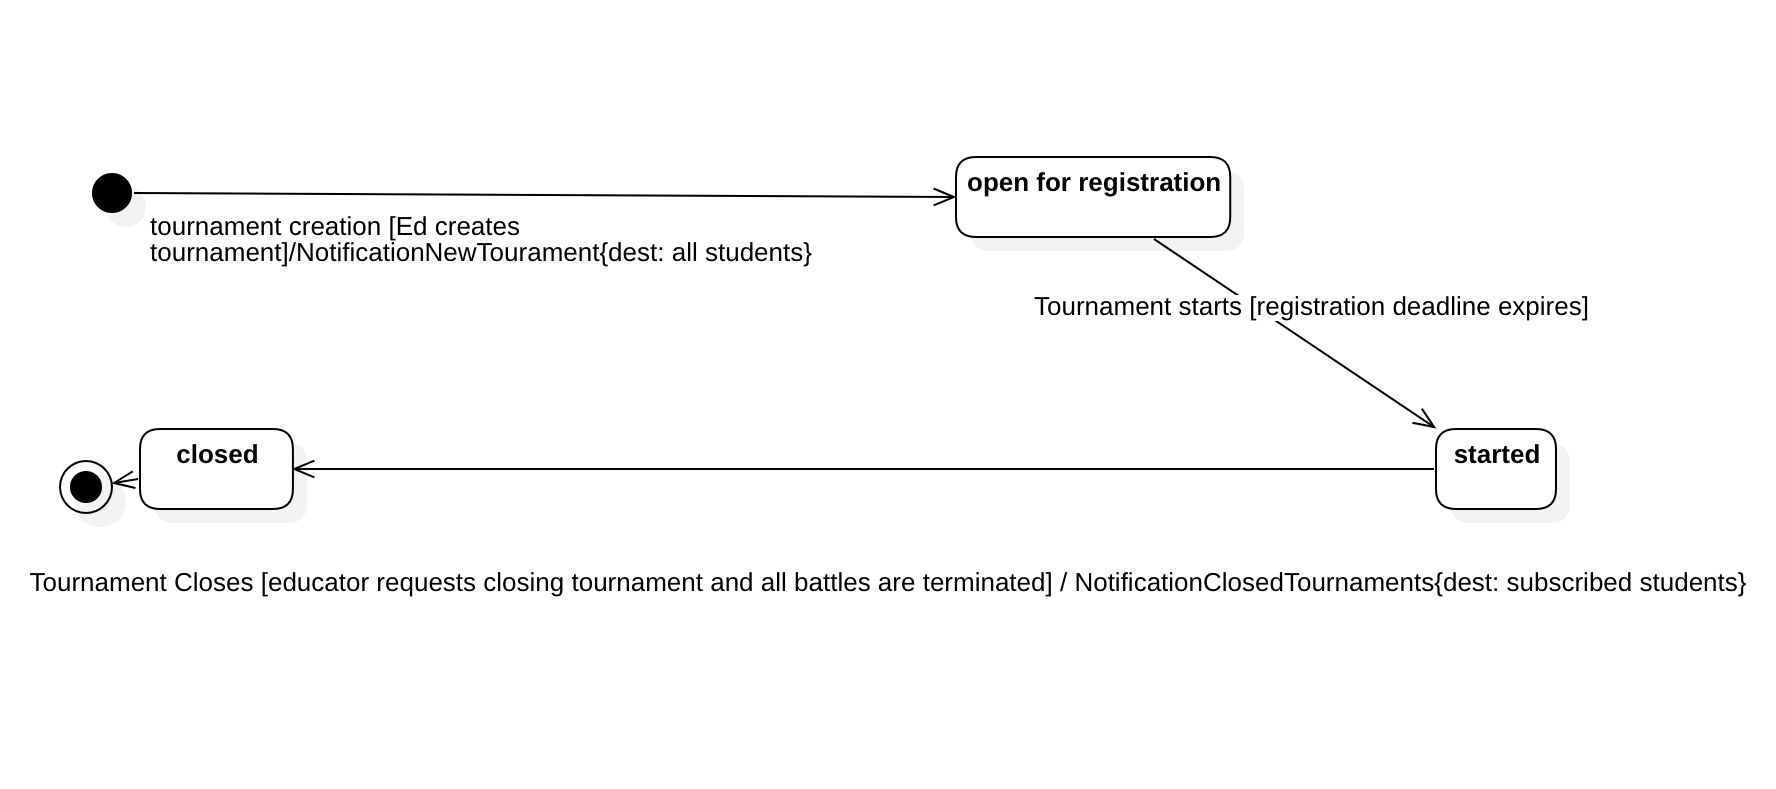
\includegraphics[width=1\textwidth]{2Overall_Description/res/st1.png}
\end{figure}

After an educator has created a tournament all the students can subscribe to it, this is the \textbf{Open for registration} state. After the registration deadline the tournament starts, student can't enroll anymore and edcucators can create battles, this is the \textbf{Started} state. When the educator that created the tournament decides it's time to close it, he can do so if there aren't ongoing battles, if he succeeds the tournament is closed (state \textbf{closed}).\\
\\
\clearpage
\textbf{Battle State Chart:}
\begin{figure}[h]
    \centering
    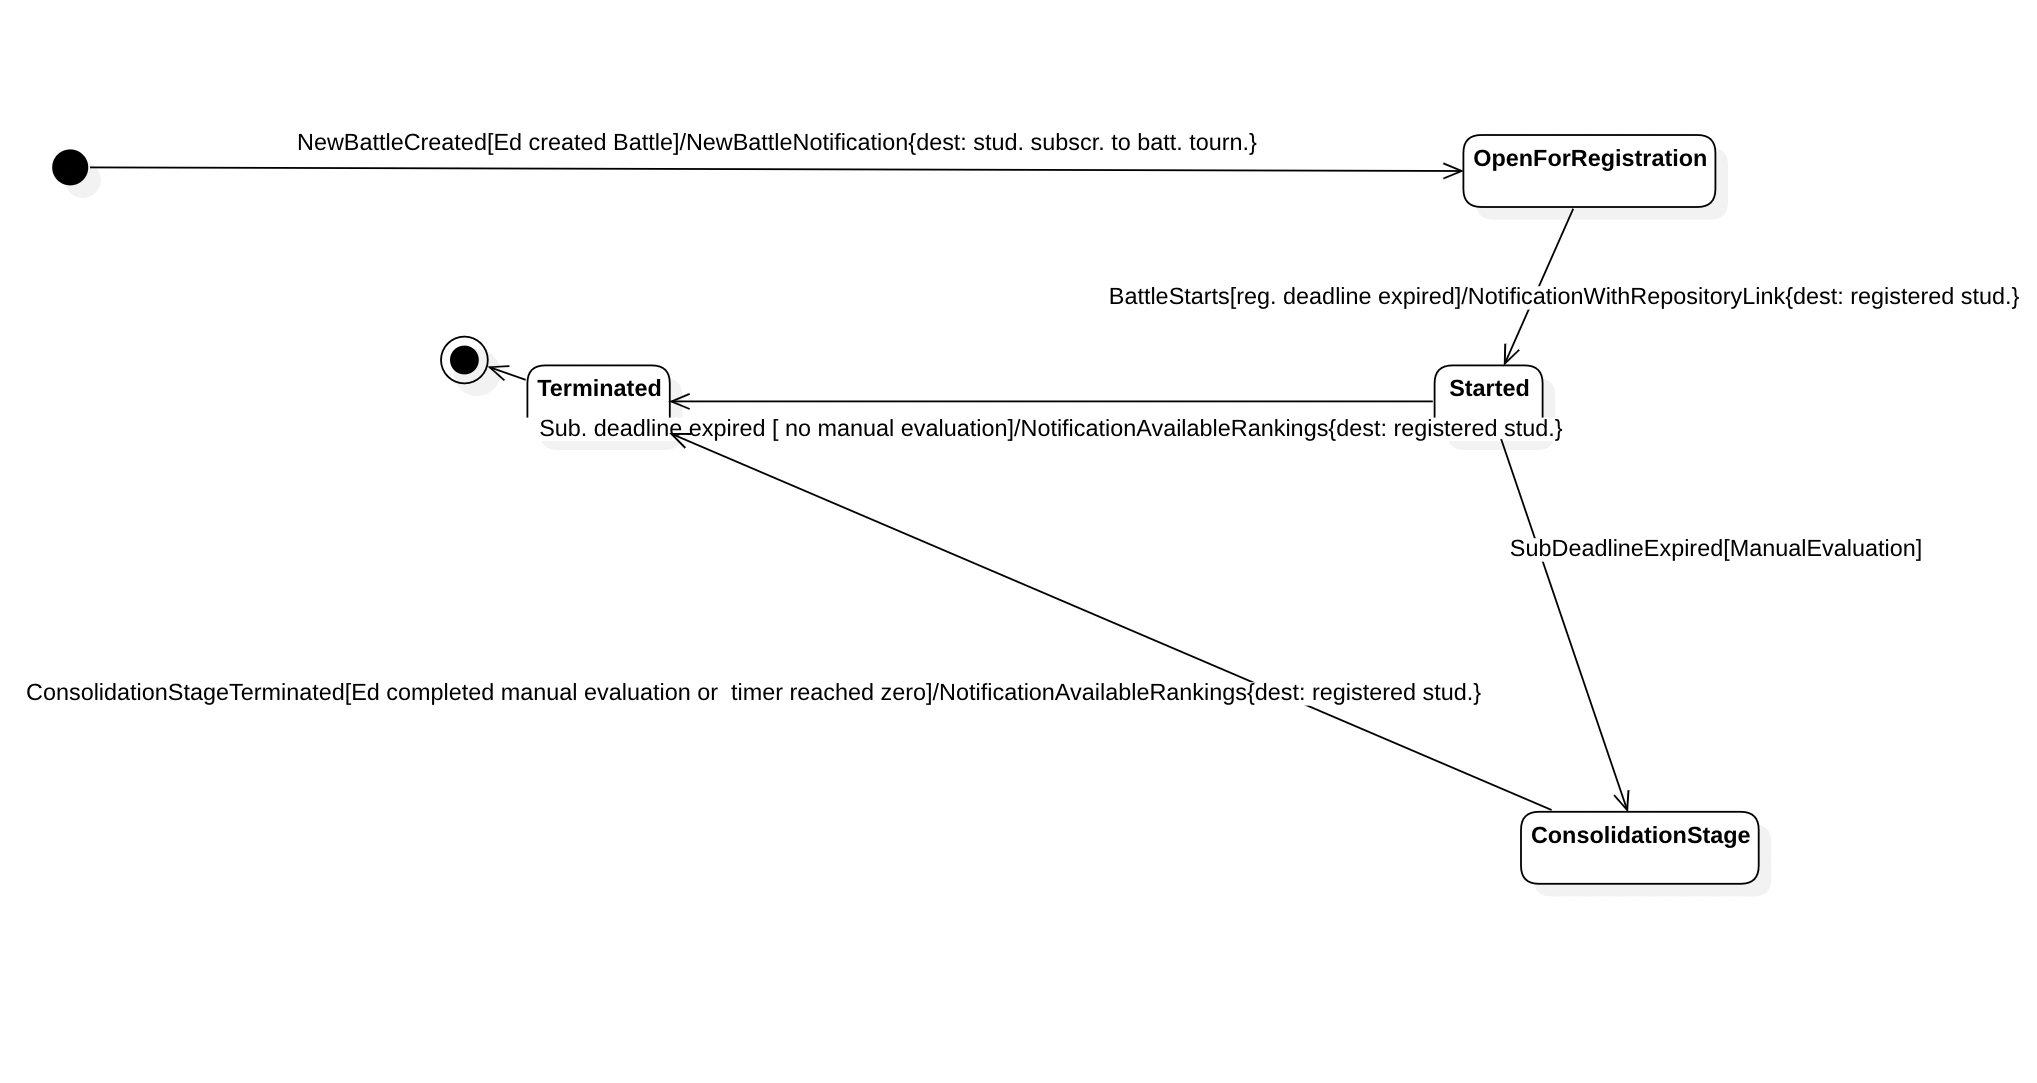
\includegraphics[width=1\textwidth]{2Overall_Description/res/stateChartBattle.png}
\end{figure}

After a battle is created students can enroll (\textbf{Open for registration} state). After the registration deadline students can't enroll anymore and a link to the battle repository is sent to all the registered students, (\textbf{Started} state). After the submission deadline, if the educator who created the battle has included a manual evaluation the Battle goes in a \textbf{Consolidation Stage} state. During the consolidation stage the educator assigns a score to each team last updated solution. The Battle goes from the consolidation stage state to \textbf{Terminated} state when the educator has finished grading all solutions, or when too much time has passed since the consolidation stage has started (fixed at 30 days). If no manual evaluation is expected, when the submission deadline expires the battle goes from the state \textbf{Started} to state \textbf{Terminated}.
\clearpage

\subsubsection{Activity Diagrams}
Here are illustrated the activity diagrams of the important workflows of CKB we wanted to highlight.\\
\\
\textbf{Computing Score Activity Diagram}\\
\begin{figure}[h]
    \clearpage
    \centering
    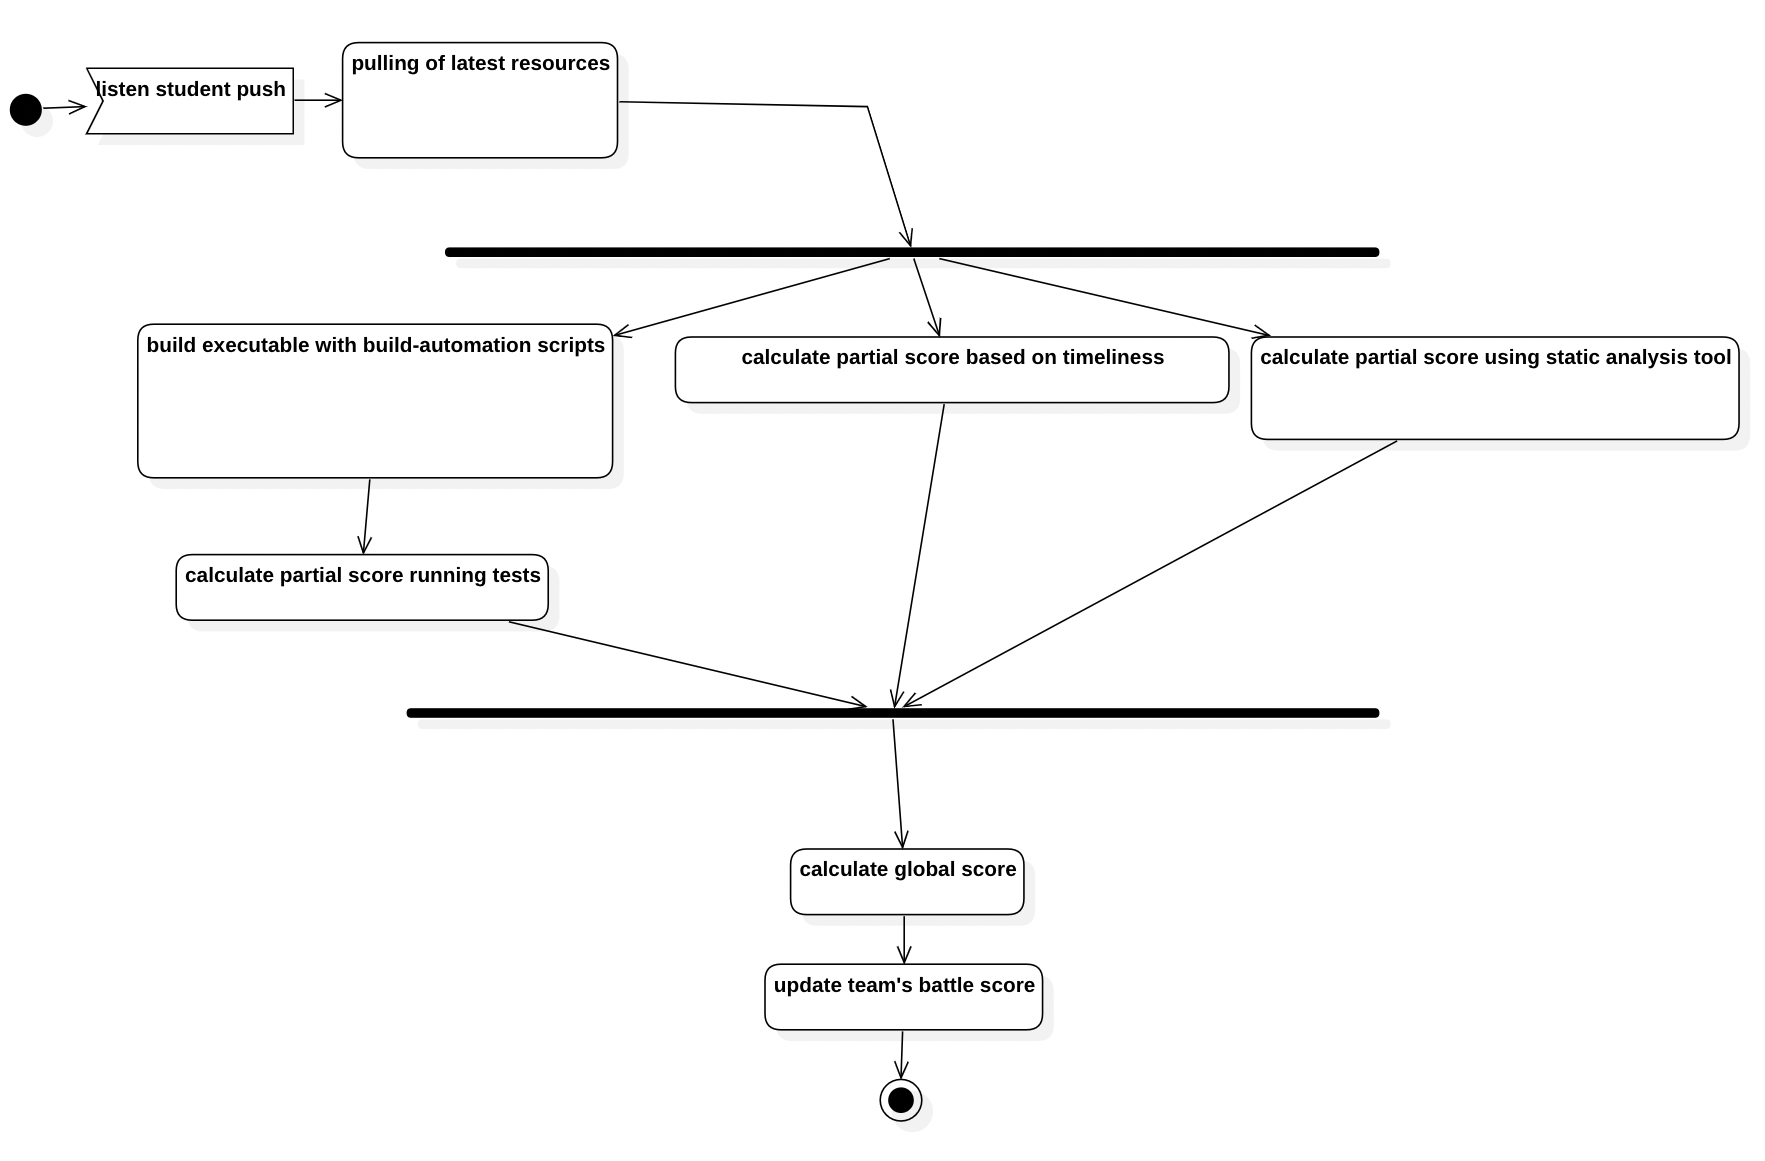
\includegraphics[width=1\textwidth]{RASD/2Overall_Description/res/newestActDgPush.png}
\end{figure}

The first activity diagram regards the process of anlayzing the correctnenss of a team's solution and the computation of it's score. The process is triggered by a push made by a student in the main branch of his ForkedRepository. Since the final score is obteined by merging results of three different analysis (static analysis, timeliness and number of test cases passed) we modeled the activities as three parallel activities.\\
\\
\newpage
\textbf{End of Battle Activity Diagram}\\
\begin{figure}[h]
    \centering
    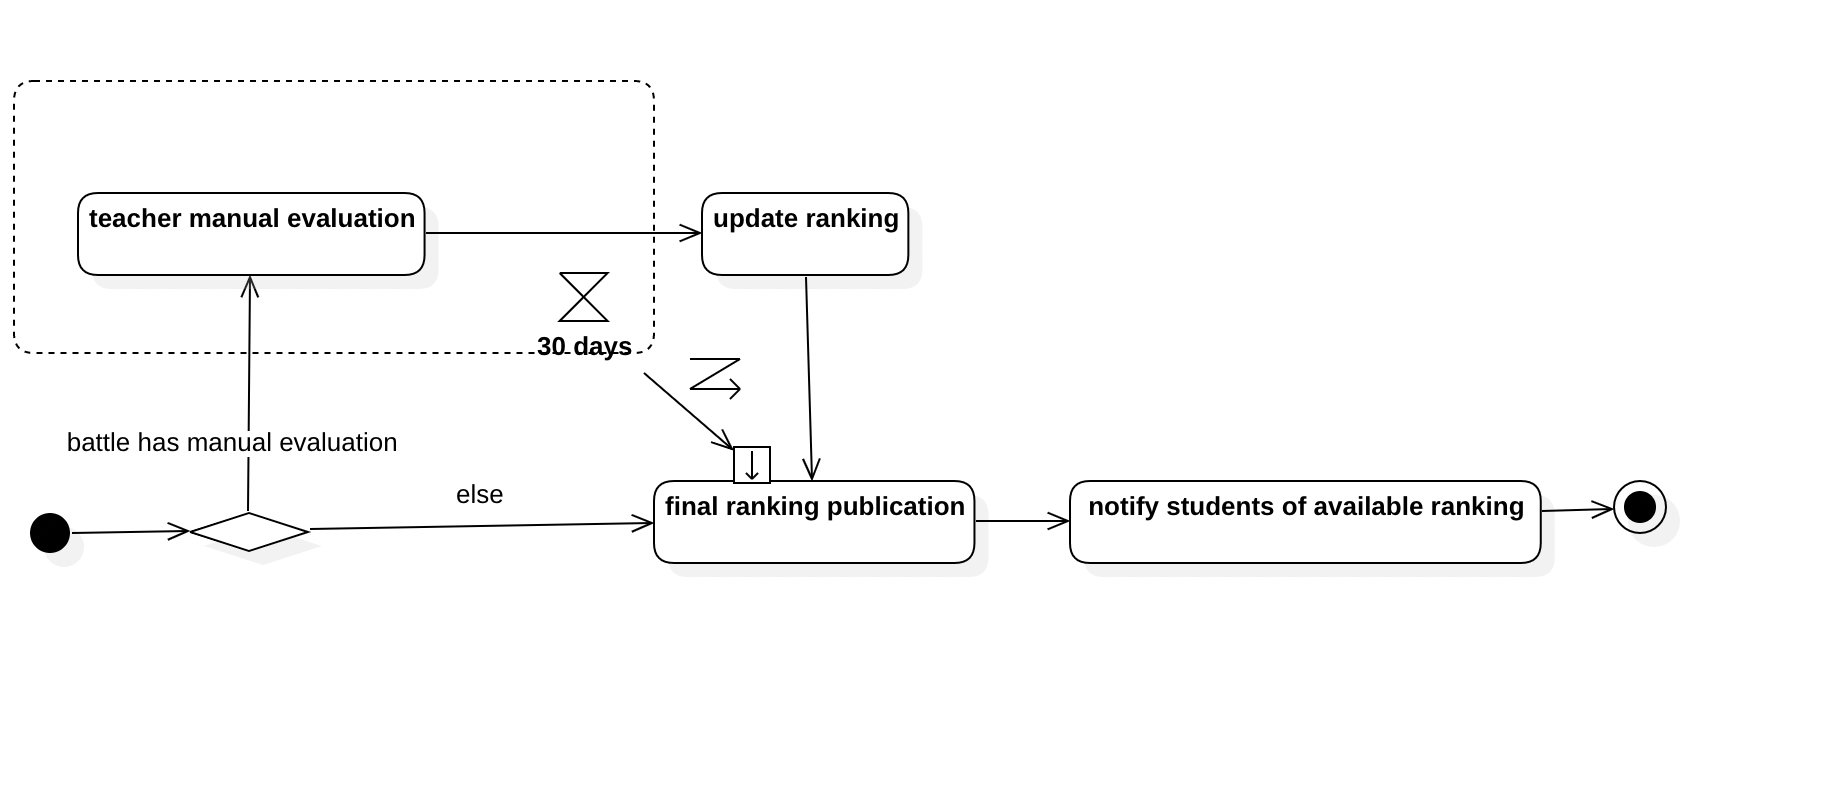
\includegraphics[width=1\textwidth]{RASD/2Overall_Description/res/ActivityDiagramEndBattle.png}
\end{figure}

The second activity diagram delineates the process of publishing the conclusive battle results, initiated upon the expiration of the battle submission deadline. The diagram is of interest because it highlights the workflow of when a battle expects a manual evaluation. The  \textbf{Manual Evaluation} activity is executed by an external actor, typically an educator. Should this activity not conclude before a predefined time, the system autonomously proceeds to publish the final results.

\clearpage
\subsection{Product Functions}
\subsubsection{Requirements}

This section shows a comprehensive list of functional requirements that \app has to meet while being developed. Functional requirements are the actions and choices that the system under analysis has to take in order to meet the stakeholders' needs.
These requirements are the result of an elicitation and abstraction process that comes from the previous sections of this document. The analysis of the relevant phenomena for the domain of interest, the validation of the stakeholders' needs by means of scenarios and the graphical illustrations provided by the several diagrams lay solid foundations for the design of the following part of the document. 

\vspace{1cm}

\renewcommand{\arraystretch}{1.9}

\begin{longtable}{|p{16.5cm}|}
	\caption*{Requirements for Goal G1}
	\\
	\hline
(R1.1) The system allows students to log in the platform using their GitHub account. \\ 
\hline
(R1.2) The system notifies all students on the platform every time a new tournament is created.\\
\hline
(R1.3) When the student requires it, the system shows the list of tournaments available on the platform for subscription (whose registration deadline hasn't passed yet). \\
\hline
(R1.4) When the student requires it, the system shows the list of tournaments the student is subscribed to.\\
\hline
(R1.5) The system allows students to subscribe to tournaments, by the end of the registration deadlines set for the tournaments.  \\
\hline
(R1.6) The system notifies all students subscribed to a tournament every time a new battle within that tournament is published.  \\
\hline
(R1.7) The system allows students subscribed to a tournament to join battle(s) within that tournament, by the end of the registration deadline set for the battle(s). \\
\hline
(R1.8) The system allows students subscribed to a tournament to join a battle of the tournament either on their own or creating teams with other students.  \\
\hline
(R1.9) The system manages all the interactions with the GitHub platform in order to allow students to submit their code solutions through GitHub.
	
\begin{minipage}[t]{\linewidth}
\begin{itemize}[nosep]
\item (R1.9.1) The system creates a new GitHub repository dedicated to a battle right after the registration deadline for that battle passes.
\item (R1.9.2) The system sends the link of the GitHub repository dedicated to a battle to all the students subscribed to that battle.
\item (R1.9.3) The system accepts notifications from GitHub in order to know when a new commit is performed by a student in any GitHub repository forked by the one created by the system itself.
\item (R1.9.4) The system pulls from the GitHub repositories of ongoing battles the new students' code solutions, every time it receives a notification from GitHub of a new commit in those repositories.\\
\end{itemize}
\end{minipage} 
\\
\hline 
(R1.10) The system calculates and then publishes the new score of a team's solution every time it receives a notification from GitHub of a new commit performed by a member of the team. \\
\hline
(R1.11) The system notifies all students participating in a battle when the final ranking of teams is available on the platform.  \\
\hline
(R1.12) The system notifies all students subscribed to a tournament when the tournament is closed by the educator who created it.\\
\hline
\end{longtable}

\vspace*{1cm}

\begin{longtable}{|p{16.5cm}|}
	\caption*{Requirements for Goal G2}\\
	\hline

(R2.1) The system allows educators to log in the platform using their GitHub account. \\
\hline
(R2.2) The system allows educators to create new tournaments.  

\begin{minipage}{\linewidth}
	\begin{itemize}[nosep]		
		\item (R2.2.1) The system allows educators to set the name of the tournament they want to create.
		\item (R2.2.2) The system allows educators to set a registration deadline for the tournament they want to create.\\
	\end{itemize}
\end{minipage}
\\
\hline
(R2.3) The system allows the educator that created a tournament to grant the permission of publishing battles within his/her tournament to other educators on the platform. \\
\hline
(R2.4) The system allows educators to create new battle(s) in the tournaments they have the permissions to do so.

\begin{minipage}{\linewidth}
	\begin{itemize}[nosep]
		\item (R2.4.1) The system allows educators to write on the platform the textual description of the battle they want to create.  
		\item (R2.4.2) The system allows educators to upload the build automation scripts designed for the battle they want to create.
		\item (R2.4.3) The system allows educators to upload the test cases designed for the battle they want to create.
		\item (R2.4.4) The system allows educators to set the minimum and maximum number of members for each team of students participating in the battle they want to create. 
		\item (R2.4.5) The system allows educators to decide whether to require a consolidation stage or not at the end of the battle they want to create. 
		\item (R2.4.6) The system allows educators to specify what evaluation criteria (reliability, security...) should be used by the system in order to compute the partial scores of the students' code solutions through an external static analysis tools. 
		\item (R2.4.7) The system allows educators to set a registration deadline for the battle they want to create.
		\item (R2.4.8) The system allows educators to set a submission deadline for the battle they want to create.  \\
	\end{itemize}
\end{minipage}\\
\hline

(R2.5) The system doesn't take into account any new code solution for a battle after the submission deadline of that battle.  \\
\hline
(R2.6) After the submission deadline of a battle and only if a consolidation stage had been requested by the educator at battle creation time, the system sets a time frame for the educator that created the battle to allow him/her to assign personal scores to the students’ code solutions.  \\
\hline
(R2.7) The system takes into account the personal scores assigned by the educator during the consolidation stage of a battle only if the educator assigned a score to all teams within the imposed time frame. \\
\hline
(R2.8) At the end of a battle and after the consolidation stage (if requested), the system automatically calculates and publishes the final rank of all teams that participated in that battle.  \\
\hline
(R2.9) When a tournament is closed, the system automatically publishes the rank of all students that participated in the tournament. \\
\hline

\end{longtable}

\vspace*{1cm}

\begin{longtable}{|p{16.5cm}|}
	\caption*{Requirements for Goal G3}\\
	\hline
	

(R3.1) The system allows students subscribed to the same tournament to invite each other in order to join battles together as a team, respecting the minimum and maximum number of students permitted for a team in the battle. \\
\hline
(R3.2) The system allows students to accept or reject invitations from other student asking to join a battle together as a team.\\
\hline
(R3.3) The system allows students to set the name of their team when they join a battle with other students.\\
\hline
(R3.4) The system calculates and then publishes the score assigned to a new code solution of a team in a battle, every time GitHub notifies the platform of a new commit performed by a member of such team. \\
\hline
(R3.5) The system constantly keeps updated the total ranking of teams for a battle, which evolves based on the new code solutions that are uploaded by students on the GitHub repository. \\
\hline
(R3.6) The system calculates and publishes the final ranking of teams when a battle ends. \\
\hline
(R3.7) The system allows only the educators and students involved in a battle to see the partial or final ranking of teams for that battle. \\
\hline
(R3.8) The system automatically calculates and keeps updated the total ranking of students subscribed to a tournament, based on the scores each student received in the battles he participated in. \\
\hline
(R3.9) The system allows all users on the platform to see the partial or final rankings of tournaments. \\
\hline
(R3.10)  The system allows educators to define customary badges (rewards) for the students participating in their tournaments, at tournament creation time. \\
\hline
(R3.11) The system assigns badges (rewards) to students that participated in a tournament, when the tournament is closed by the educator that created it. \\
\hline
(R3.12) The system allows all users on the platform to search for the personal profile of a student and see the corresponding account. \\
\hline
(R3.13) The system allows all users on the platform to see the list of badges owned by a student for the tournaments s/he participated in. \\
\hline

\end{longtable}

\clearpage
\subsection{User Characteristics}
\subsubsection{Student}
\subsubsection{Educator}
The educator is an individual with advanced education in programming, equipped with the proficiency to teach effectively. This is especially necessary in order to write the build automation scripts and test cases that have to be uploaded on \app every time a new battle is created. Additionally, the educator has the capability of thinking and designing code kata battles, adjusting them to specific difficulty levels suitable for students.








\subsection{Assumptions, Dependencies and Constraints}
\subsubsection{Domain Assumptions}
\begin{enumerate}[label=D\arabic*]
		\item The GitHub platform is up and running and provides all the functionalities that are expected by \app to work correctly (creation of repositories, forking of repositories, notification system...).
		\item All users of \app have a personal GitHub account or are able to create a new one.
		\item Student correctly forks the main branch of the GitHub repository dedicated to a battle in order to submit his/her code solutions.
		\item Student correctly writes the automated GitHub workflow to send notifications from GitHub to the system every time a commit is performed on the forked repository.
		\item Educator correctly writes the build automation scripts for the battles s/he creates on the platform.
		\item Educator correctly writes the test cases for the battles s/he creates on the platform.
		\item The network allows notifications sent by the application to successfully reach the users, as well as the interaction with the GitHub platform to work correctly.
	\end{enumerate}
\clearpage
\clearpage
\section{Specific Requirements}
(R1.1) The system allows students that don't have an account to sign up for the first time on the platform.  \\
(R1.2) The system allows students that already have an account to log in the platform.\\
(R1.3) The system notifies all students that have an account on the platform every time a new tournament is created.\\
(R1.4) The system shows to a student the list of tournaments available on the platform, including closed tournament, the ones the student is already subscribed to and the ones s/he can subscribe to. \\
(R1.5) The system allows students to join the tournaments they’re interested in, by the end of the registration deadlines set for the tournaments.  \\
(R1.6) The system notifies all students subscribed to a tournament every time a new battle within that tournament is published.  \\
 (R1.7) The system allows students subscribed to a tournament to join battle(s) within that tournament, by the end of the registration deadline set for the battle(s). \\
 (R1.8) The system allows students subscribed to a tournament to join a battle of the tournament either on their own or creating teams with other students.  \\
 (R1.10) The system sends the link of the GitHub repository dedicated to a battle to all the students subscribed to that battle. \\
 (R1.11) The system notifies all students participating in a battle when the battle terminates and the final ranking of teams is available on the platform.  \\
 (R1.12) The system notifies all students subscribed to a tournament when the tournament is closed by the educator who created it.
 (R1.13) The system creates a new GitHub repository dedicated to a battle when the registration deadline for that battle passes. \\
(R1.14) The system accepts notifications from GitHub in order to know when a new commit is performed by a student in any GitHub repository dedicated to an ongoing battle.  \\
(R1.15) The system pulls from the GitHub repositories of ongoing battles the new students' code solutions, every time it receives a notification from GitHub of a new commit in those repositories.  \\
(R1.16) The system recalculates and then publishes the new score of a team's solution every time it receives a notification from GitHub of a new commit performed by a member of the team.  \\
(R2.1) The system allows educators that don’t have an account to sign up for the first time on the platform. \\
(R2.2) The system allows educators that already have an account to log in the platform. \\
(R2.3) The system allows educators to create new tournaments.  \\
(R2.4) The system allows educators to set a registration deadline for the tournament(s) they want to create  \\
(R2.6) The system allows the educator that created a tournament to grant the permission of publishing battles within his/her tournament to other educators on the platform. \\
(R2.7) The system allows educators to create new battle(s) in the tournaments they have the permissions to do so \\
(R2.8) The system allows educators to upload on the platform the textual description of a battle they want to create.  \\
(R2.9) The system allows educators to set a minimum and maximum number of members for each team of students participating in the battle they want to create  \\
(R2.10) The system allows educators to declare whether to require a consolidation stage or not at the end of the battle they want to create.  \\
(R2.11) The system allows educators to specify what parameters of evaluation (reliability, security...) should be used by the system in order to compute the scores of the students' code solutions through static analysis external tools.  \\
(R2.12) The system allows educators to set a registration deadline for the battle they want to create.  \\
(R2.13) The system allows educators to set a submission deadline for the battle they want to create.  \\
(R2.14) The system doesn't take into account any new code solution for a battle after the submission deadline of that battle.  \\
(R2.15) After the submission deadline of a battle and only if a consolidation stage had been requested by the educator at battle creation time, the system sets a time frame for the educator that created the battle to allow him/her to assign personal scores to the students’ code solutions.  \\
(R2.16) The system takes into account the personal scores assigned by the educator during the consolidation stage of a battle only if the educator assigned a score to all teams within the imposed time frame. \\
(R2.17) At the end of a battle and after the consolidation stage (if requested), the system automatically calculates and publishes the final rank of all teams that participated in that battle.  \\
(R2.18) When a tournament is closed, the system automatically publishes the rank of all students that participated in the tournament. \\
(R3.1) The system allows students subscribed to the same tournament to invite each other in order to join battles as a team, respecting the minimum and maximum number of students permitted for a team in the battle. \\
(R3.2) The system calculates and then publishes the score assigned to a new code solution of a team in a battle, every time GitHub notifies the platform of a new commit performed by a member of such team. \\
(R3.3) The system constantly keeps updated the total ranking of teams for a battle, which evolves based on the new code solutions that are uploaded by students on the GitHub repository. \\
(R3.4) The system calculates and publishes the final ranking of teams when a battle ends. \\
(R3.5) The system allows only the educators and students involved in a battle to see the partial or final ranking of teams for that battle. \\
(R3.6) The system automatically calculates and keeps updated the total ranking of students subscribed to a tournament, based on the scores each student received in the battles he participated in. \\
(R3.7) The system allows all users on the platform to see the partial or final rankings of tournaments. \\
(R3.8)  The system allows educators to define customary badges (rewards) for the students participating in their tournaments, at tournament creation time. \\
(R3.9) The system assigns badges (rewards) to students that participated in a tournament when the tournament is closed by the educator that created it. \\
(R3.10) The system allows all users on the platform to search for the personal profile of a student and see the corresponding page. \\
(R3.11) The system allows all users on the platform to see the list of badges owned by a student for the tournaments s/he participated in. \\
\subsection{External Interface Requirements}
\subsubsection{User Interface}
This section is dedicated to the illustration of some mockups of the most relevant graphical user interfaces that \app uses to interact with external users (educators and students). 
The aim of these representations is to specify the logical characteristics of the presented interfaces as well as introducing some guidelines on the style and look that the final product will have. This information can be used in order to shape the design of the \app platform in more advanced stages of the development.
 
\vspace{1cm}

\begin{minipage}{\linewidth}
	\textbf{Log In Interface}
  \begin{center}
  \includegraphics[page=1,width=0.7\linewidth,keepaspectratio]{3Specific_Requirements/res/UI_Mockup}

  \end{center}
    Log In Interface for both Educators and Students, who can access \app through their GitHub account by clicking on the button "Login Through GitHub"
\end{minipage}

\vspace{1cm}

\begin{minipage}{\linewidth}
	\textbf{Home Page Student}
	\begin{center}
		\includegraphics[page=2,width=0.7\linewidth,keepaspectratio]{3Specific_Requirements/res/UI_Mockup}
		
	\end{center}
	Home page for a student, in which it is possible to:
	\begin{itemize}
		\item See personal profile of the student, with a customary image.
		\item See the list of badges earned by the student in tournaments s/he participated in.
		\item Ask for the list of tournaments the student is subscribed to.
		\item Subscribe to a new tournament with the "Join Tournament" button.
		\item Search for a user on the platform (with the magnifying glass in the top right corner). 
	\end{itemize}
\end{minipage}

\vspace{1cm}

\begin{minipage}{\linewidth}
	\textbf{Home Page Educator}
	\begin{center}
		\includegraphics[page=3,width=0.7\linewidth,keepaspectratio]{3Specific_Requirements/res/UI_Mockup}
		
	\end{center}
	Home page for an educator, in which it is possible to:
	\begin{itemize}
		\item See personal profile of the educator, with a customary image.
		\item Ask for the list of tournaments the educator created (or has permissions to publish battles in), with the "My Tournaments" button.
		\item Create a new battle with the "New Battle" button. 
		\item Create a new tournament with the "New Tournament" button.
		\item Search for a user on the platform (with the magnifying glass in the top right corner). 
	\end{itemize}
\end{minipage}

\vspace{1cm}

\begin{minipage}{\linewidth}
	\textbf{Tournament Creation Form}
	\begin{center}
		\includegraphics[page=4,width=0.7\linewidth,keepaspectratio]{3Specific_Requirements/res/UI_Mockup}
		
	\end{center}
 	This interface pops up when the educator clicks on "New Tournament" from the home page. Thanks to this form, all relevant parameters for the creation of a tournament can be set.

\end{minipage}

\vspace{1cm}

\begin{minipage}{\linewidth}
	\textbf{Tournament Creation Form}
	\begin{center}
		\includegraphics[page=5,width=0.7\linewidth,keepaspectratio]{3Specific_Requirements/res/UI_Mockup}
		
	\end{center}
	This interface pops up when the educator clicks on "New Tournament" from the home page. Thanks to this form, all relevant parameters for the creation of a tournament can be set.
	
\end{minipage}
\subsubsection{Hardware Interfaces}
The system offers the services described in section 2 via different hardware interfaces as CodeKataBattle services are provided via a web page and via a mobile application.
To access the service offered by the system both kind of users are required to have either a device with an internet connection, to access the web page, or the mobile application.
Students are also required to have access to a computer with internet connection to be able to access the GitHub page containing the material for the battle and to be able to manage their GithHub projects.

\subsubsection{Software Interfaces}
The system requires some software interfaces in order to provide its services. Below are reported the most significant:
\begin{itemize}
    \item GitHub API Integration : The system communicates with external APIs to allow the creation of GithHub repositories for each battle
\end{itemize}
\subsection{Functional Requirements}
\subsubsection{Use Case Diagrams}

\includegraphics*[width=18cm,keepaspectratio]{UseCaseDiagram1}
\vspace*{3cm}
\includegraphics*[width=12cm,keepaspectratio]{UseCaseDiagram2}
\subsubsection{UseCases}

\renewcommand{\arraystretch}{1.9}

	

    \begin{longtable}{|p{3cm}p{14cm}|}
    \multicolumn{2}{l}{\textbf{[UC1] - EducatorLogIn} }\\
        \hline 
         Name & EducatorLogIn \\
        \hline 
        Actors & Educator, GitHub. \\
        \hline
        Entry Condition & Educator has opened \app on his/her laptop. \\
        \hline
        Event Flow &  
        	1 - \app shows the log in interface with the button to sign in with a GitHub account.

        	2 - Educator clicks on the button to sign in using his/her GitHub account.

        	3 - \app redirects the educator to the GitHub login page.
        	
        	4 - Educator inserts his/her GitHub credentials and confirms.\\
        \hline
        Exit Condition & \app shows the initial (home) page of the application for an educator.  \\
        \hline
        Exceptions & 
        	1 - Educator inserts wrong credentials to access his/her GitHub account: the GitHub authentication page will return an error to the educator, asking him/her to retry.\\
        \hline
      
    \end{longtable}
      
	
	
	\begin{longtable}{|p{3cm}p{14cm}|}
		\multicolumn{2}{l}{\textbf{[UC2] - StudentLogIn}}\\
		\hline
		Name & StudentLogIn \\
		\hline
		Actors & Student, GitHub. \\
		\hline
		Entry Condition & Student has opened \app on his/her laptop. \\
		\hline
		Event Flow &  
		
		1 - \app shows the log in interface with the button to sign in with a GitHub account.
		
		2 - Student clicks on the button to sign in using his/her GitHub account.
		
		3 - \app redirects the student to the GitHub login page.
		
		4 - Student inserts his/her GitHub credentials and confirms.
		\\
		\hline
		Exit Condition & \app shows the initial (home) page of the application for an student.  \\
		\hline
		Exceptions & 
		1 - Student inserts wrong credentials to access his/her GitHub account: the GitHub authentication page will return an error to the student, asking him/her to retry.\\
		\hline
    
    \end{longtable}
    
    
      \begin{longtable}{|p{3cm}p{14cm}|}
      	\multicolumn{2}{l}{\textbf{[UC3] - CreateTournament}}\\
        \hline
         Name & CreateTournament \\
        \hline
        Actors & Educator, Student. \\
        \hline
        Entry Condition & Educator is logged in the \app platform.  \\
        \hline
        Event Flow &  
        	1 - Educator clicks on the button to create a new tournament.
        	 
        	2 - \app shows the form to fill with the information for the tournament to be created.
        	
        	3 - Educator types in the name of the tournament.
        	
        	4 - Educator writes down a description of the tournament.
        	
        	5 - Educator defines the registration deadline by which students are asked to register for the tournament if interested.
        	
        	6 - Educator defines the badges (rewards) to be assigned to students at the end of the tournament based on some customary achievements.
        	
        	7 - Educator confirms the information filled in the form.
        	
        	8 - \app shows the initial page of the tournament to the educator.
        	
        	8 - \app sends a notification to all the students on the platform to inform them of the new tournament available.\\
      
        
        \hline
        Exit Condition & The new tournament is added to the list of tournaments created by the educator and all users on the platform can see the new tournament. \\
        \hline
        Exceptions &
        1 - The registration deadline set by the educator is on the same day or before the day in which the educator is trying to create the new tournament: the system does not allow the educator to confirm the creation of the tournament and reports an error message.
        
        2 - Educator confirms the form to create the new tournament leaving some mandatory information unspecified: in this case \app will return an error message to the educator stating that some information is missing and the tournament cannot be created.\\
        \hline
        Special Requirements & Mandatory data in the tournament creation form is composed of name and registration deadline of the tournament.
        \\
        \hline
      
    \end{longtable}

    
      \begin{longtable}{|p{3cm}p{14cm}|}
      	\multicolumn{2}{l}{ \textbf{[UC4] - CreateBattle}}\\
        \hline
         Name & CreateBattle \\
        \hline
        Actors & Educator, Student. \\
        \hline
        Entry Condition & Educator is logged in the \app platform and has the permissions to publish a battle in the tournament which the battle will reside in. S/he has already written the build automation scripts and test cases for the battle to be created. \\
        \hline
        Event Flow & 
        	1 - Educator clicks on the button to create a new battle from the home page of \app.
        	
        	2 - \app displays the entire list of tournaments in which the educator has permissions to publish battles.
        	
        	3 - Educator selects the tournament in which s/he wants to create the new battle.
        	
        	4 - \app shows the form to fill in with all the relevant data associated with the battle.
        	
        	5 - Educator types in the name of the battle.
        	
        	6 - Educator writes down the textual description of the battle.
        	
        	7 - Educator uploads the build automation scripts related to the battle.
        	
        	8 - Educator uploads the test cases related to the battle.
        	
        	9 - Educator sets the registration deadline for the battle, by which students are asked to join if interested.
        	
        	10 - Educator sets the submission deadline for the battle, after which \app stops accepting additional solutions to the battle.
        	
        	11 - Educator sets the minimum and maximum number of students allowed per team.
        	
        	12 - Educator selects the aspects on which \app automatically evaluates the students' code solutions, leveraging an external static analysis tool. For instance maintainability, security...
        	
        	13 - Educator specifies whether a consolidation stage for personal evaluation of the students' code solutions is required at the end of the battle.
        	
        	14 - Educator clicks on the button to confirm the data inserted in the form.
        	
        	15 - \app shows the educator the presentation page of the newly created battle.
        	
        	16 - \app sends a notification to all the students subscribed to the tournament in which the battle has been created, informing them of the new battle available.
        \\
        \hline
        Exit Condition & The new battle is added on the list of battles created by the educator and students are able to see this new battle in the tournament in which it resides. \\
        \hline
        Exceptions & 
        
        1 - The registration deadline set by the educator is on the same day or before the day in which the educator is trying to create the new battle: the system does not allow the educator to confirm the creation of the battle and reports an error message.
        
       	2 - The submission deadline set by the educator is on the same day or before the day of the registration deadline: the system does not allow the educator to confirm the creation of the tournament and reports an error message.
        
        3 - Educator confirms the creation of the battle without uploading either the build automation scripts or the test cases for the battle: the system doesn't create any new battle and reports an error message to the educator stating the reason why the battle cannot be instantiated.
        
        4 - Educator confirms the creation of the battle without specifying some mandatory information for the battle: the system doesn't create any new battle and reports an error message to the educator stating the reason why the battle cannot be instantiated.\\
        \hline
        Special Requirements & Mandatory data in the battle form include the battle's name, the textual description of the problem to be solved, the registration and submission deadlines, the minimum and maximum number of students per team.\\
         \hline
      
    \end{longtable}
      
     \begin{longtable}{|p{3cm}p{14cm}|}
     	\multicolumn{2}{l}{\textbf{[UC5] - GrantPermissions}}\\
        \hline
        Name & GrantPermissions \\
        \hline
        Actors & Educator. \\
        \hline
        Entry Condition & Educator A is logged in the system. Educator A created a tournament on the platform. \\
        \hline
        Event Flow &  
        1 - Educator A selects from the home page of \app the button to visualize the list the tournaments that s/he created.
        
        2 - \app displays the list of tournaments created by educator A.
        
        3 - Educator A clicks on the tournament in which s/he wants to grant permissions to educator B.
        
        4 - \app opens the description page of the selected tournament.
        
        5 - Educator A clicks on the button to grant the permissions to publish battles to another educator in the tournament.
        
        6 - \app displays an interface to search for an educator by username.
        
        7 - Educator A types in educator B's username, finds him/her and confirms the choice.
        
        8 - \app sends a request to educator B to inform him/her of the possibility to publish battles in A's tournament.
        
        9 - Educator B accepts the request.
        \\
        \hline
        Exit Condition & The system adds the tournament to the list of tournaments in which educator B has permissions to publish battles.\\
        \hline
        Exceptions & 
        1 - Educator A tries to grant publishing permissions to educator B who already had permissions on that tournament: \app doesn't modify anything on B's account and reports to A that B already had publishing permissions on that tournament.
        
        2 - Educator A tries to grant publishing permissions to educator B on a closed tournament: \app doesn't modify anything on B's account and reports to A the tournament is already terminated.
        \\
        \hline
      
    \end{longtable}

    
      \begin{longtable}{|p{3cm}p{14cm}|}
      	\multicolumn{2}{l}{\textbf{[UC6] - SubscribeToTournament}}\\
        \hline
        Name & SubscribeToTournament \\
        \hline
        Actors & Student. \\
        \hline
        Entry Condition & The student is logged in the system.\\
        \hline
        Event Flow &  
        1 - \app displays the list of available tournaments on the platform in the home page.
        
        2 - Student browses the list of available tournaments and reads some of their descriptions to get an idea on them.
        
        3 - Student clicks on the tournament wants to subscribe to.
        
        4 - \app shows the home page of the selected tournament.
        
        5 - Student clicks on the button to subscribe to the tournament and confirms his choice.
        \\
        \hline
        Exit Condition & The system adds the tournament to the list of tournaments the student is subscribed to. \\
        \hline
        Exceptions & 
        1 - Student tries to subscribe to a tournament whose registration deadline has already passed: \app reports an error message to the student stating that it is not possible to carry out the operation.
        \\
        \hline
    \end{longtable}

   

      
     \begin{longtable}{|p{3cm}p{14cm}|}
     	\multicolumn{2}{l}{\textbf{[UC7] - JoinBattleAlone}}\\
        \hline
        Name & JoinBattleAlone \\
        \hline
        Actors & Student. \\
        \hline
        Entry Condition & The student is logged in the platform and is subscribed to the tournament in which the battle s/he wants to join resides.\\
        \hline
        Event Flow &  
        1 - Student opens the list of tournaments s/he's subscribed to from the home page of \app.
        
        2 - \app displays the list of tournaments the student is subscribed to.

        3 - Student clicks on the tournament in which the battle s/he wants to join resides.

        4 - \app shows the home page of the selected tournament.
        
        5 - Student selects the battle s/he wants to join and clicks on it.

        5 - \app shows the description page of the selected battle with the button to join it.
        
        6 - Student clicks the button to join the battle.
        
        7 - \app shows the interface for joining a battle, in which it is possible to decide whether to participate as a single player or with other students as a team.
        
        8 - Students opts for participating on his/her own and confirms the choice.
        
        \\
        \hline
        Exit Condition & \app adds the battle to the list of battles the student is taking part to. \\
        \hline
        Exceptions & 
        1 - Student tries to join a battle whose registration deadline has passed: \app shows an error message stating that it is not possible to carry out that operation and doesn't allow the student to join the battle.
        
        2 - Student tries to join a battle in a tournament s/he is not subscribed to: \app doesn't allow this operation and reports a warning message stating that it is necessary to first subscribe to the tournament in order to participate in its battles.
        \\
        \hline    
    \end{longtable}

   
	
	\begin{longtable}{|p{3cm}p{14cm}|}
		\multicolumn{2}{l}{\textbf{[UC8] - JoinBattleAsTeam}}\\
		\hline
		Name & JoinBattleAsTeam \\
		\hline
		Actors & Student. \\
		\hline
		Entry Condition & Students A, B, C are logged in the platform and are all subscribed to the tournament in which the battle they want to join resides.\\
		\hline
		Event flow &  
		1 - Student A opens the list of tournaments s/he's subscribed to from the home page of \app.
		
		2 - \app displays the list of tournaments the student is subscribed to.
		
		3 - Student clicks on the tournament in which the battle s/he wants to join resides.
		
		4 - \app shows the home page of the selected tournament.
		
		5 - Student selects the battle s/he wants to join and clicks on it.
		
		5 - \app shows the description page of the selected battle with the button to join it.
		
		6 - Student clicks the button to join the battle.
		
		7 - \app shows the interface for joining a battle, in which it is possible to decide whether to participate as a single player or with other students as a team.
		
		8 - Students opts for participating to the battle as a team.
		
		9 - \app shows an interface in which it is possible to search for other students by username to invite them in the team.
		
		10 - Student A types in B and C's usernames and selects them on the interface.
		
		11 - \app sends a request to students B and C asking them to participate in the team created by A.
		
		12 - Students B and C accept the request from their accounts.
		
		\\
		\hline
		Exit condition & \app adds the battle to the list of battles in which A participates, as well as to the list of battles in which B participates and C participates. \app also creates a new team grouping A, B and C together.\\
		\hline
		Exceptions & 
		1 - Student A tries to join a battle whose registration deadline has passed: \app shows an error message stating that it is not possible to carry out that operation and doesn't allow the student to join the battle.
		
		2 - Student A tries to join a battle in a tournament s/he is not subscribed to: \app doesn't allow this operation and reports a warning message stating that it is necessary to first subscribe to the tournament in order to participate in its battles.
		
		3 - Student A tries to invite a student that is not subscribed to the tournament in which the battle resides: \app won't allow this action by limiting the search space for the students to invite to the set of students subscribed to the tournament in which the battle resides.
		
		4 - Students B or C do not accept the request to join the team before the registration deadline of the battle: \app excludes them from the battle. The request is no longer valid.
		
		\\
		\hline

\end{longtable}


    \begin{longtable}{|p{3cm}p{14cm}|}
    	\multicolumn{2}{l}{\textbf{[UC9] - CreateGitHubRepository }}\\
    
        \hline
        Name & CreateGitHubRepository \\
        \hline
        Actors & GitHub, Student. \\
      \hline 
        Entry Condition &  There is a battle on \app whose registration deadline has just passed.  \\ 
       \hline 
        Event Flow & 
        
        1 - \app sends a request to GitHub to generate a new repository dedicated to the battle whose registration deadline has just passed. 
        
        2 - GitHub creates the new repository.
        
        3 - GitHub sends back a confirmation message to \app.
        
        4 - \app sends a notification to all the students who joined the battle to inform them that the battle they're subscribed to is now open and it is possible to submit code solutions through GitHub. The system also includes the link to the remote GitHub repository in the notification message.\\
        \hline
        Exit Condition &  All students subscribed to the battle receive the notification and are able to start pushing code solutions for the ongoing battle. \\
        \hline
        Exceptions & 
        1 - GitHub doesn't respond to the request and doesn't create the new repository: \app sends again the request after waiting for a fixed time interval.
        \\
        \hline

      
    \end{longtable}

    
   \begin{longtable}{|p{3cm}p{14cm}|}
   	\multicolumn{2}{l}{\textbf{[UC10] - PushSolutionGitHub} }\\
   	\hline 
   	Name & PushSolutionGitHub \\
   	\hline 
   	Actors & Student, GitHub. \\
   	\hline
   	Entry Condition & Student is logged in the system and has already joined a battle that is ongoing (the registration deadline is passed, while the submission deadline hasn't). \\
   	\hline
   	Event Flow &  
   	1 - Student pushes a new code solution on the GitHub repository that s/he forked from the main GitHub repository dedicated to the battle.
   	
   	2 - GitHub sends a notification to \app with the information relative to the new commit performed by the student.
   	
   	3 - \app downloads the new code solution from GitHub.
   	
   	4 - \app computes the score to assign to the new code solution (see UC11).
   	
   	5 - \app shows on the platform the score assigned to the new solution.
   	
   	6 - \app updates the ranking of teams in the battle accordingly to the student's new score.\\
   	\hline
   	Exit Condition & The student is able to see on \app the score of his/her solution and the new ranking of the battle.  \\
   	\hline
   	Exceptions & -\\
   	
   	\hline
   	
   \end{longtable}
   
   \begin{longtable}{|p{3cm}p{14cm}|}
   	\multicolumn{2}{l}{\textbf{[UC11] - CalculateScore} }\\
   	\hline 
   	Name & CalculateScore \\
   	\hline 
   	Actors & StaticAnalysisTool. \\
   	\hline
   	Entry Condition & A student has just pushed a new code solution on his/her GitHub repository linked to a battle, \app has received the notification from GitHub and downloaded the code of the student to be evaluated. \\
   	\hline
   	Event Flow &  
   	1 - \app uses the build automation scripts to build the student's code solution.
   	
   	2 - \app runs the test cases on the student's solution and counts how many of them are passed.
   	
   	3 - \app calculates the time went by from the beginning of the battle to the moment in which the solution was submitted and stores the information.
   	
   	4 - \app leverages the StaticAnalysisTool to evaluate the student's solution based on some criteria (such as maintainability, security...) defined by the educator that created the battle at battle creation time.
   	
   	5 - \app calculates the total score (between 0 and 100) to assign to the student's solution based on the information gathered at points 2, 3, 4.\\
   	\hline
   	Exit Condition & \app saves the total score computed for the student's solution  \\
   	\hline
   	Exceptions & 
   	1 - The building process of the code solution fails: \app terminates the computation and assigns a score of 0 to the solution. \\
   	\hline
   	
   \end{longtable}
    
     \begin{longtable}{|p{3cm}p{14cm}|}
     	\multicolumn{2}{l}{\textbf{[UC10] - EvaluateSolutions }}\\
        \hline
        Name & EvaluateSolutions \\
        \hline
        Actors & Educator. \\
        \hline
        Entry Condition &  Educator is logged in \app. Educator has already created a battle and required a consolidation stage at the end of the battle. The submission deadline of the battle has just passed. \\
        \hline
        Event Flow &  
        1 - Educator navigates on the system to the battle for which the consolidation stage has to be carried out and clicks on the button to assess the teams' solutions.
        
        2 - \app shows an interface in which for each team participating in the battle it is possible to specify a score to assign to it. On the interface there is also a timer illustrating the maximum amount of time to complete the task.
        
        3 - Educator reads the teams' solutions one by one and inputs in the system the corresponding scores.
        
        4 - After having assessed all the solutions, the educator confirms his/her choices. 
        \\

        \hline
        Exit Condition &  \app saves the scores assigned by the educator in order to calculate the final ranking for the battle.
        
        \\
        \hline
        Exceptions & 
        1 - Educator closes the consolidation stage interface before having assessed all teams' solutions: \app won't publish any final ranking yet and will save the scores assigned so far by the educator.
        
        2 - Educator doesn't complete the task of assigning personal scores before the timer goes off: \app will discard all the scores assigned by the educator and will base the final ranking only on the automatic evaluations performed during the battle.
        \\
        \hline
     
    \end{longtable}
    
    
   
    
     \begin{longtable}{|p{3cm}p{14cm}|}
     	\multicolumn{2}{l}{\textbf{[UC11] - TerminateBattle}}\\
        \hline
         Name & TerminateBattle \\
        \hline
        Actors & Educator, Student. \\
        \hline
        Entry Condition & There is a battle created on \app whose submission deadline has just passed. \\
        \hline
        Event Flow &  
        1 - \app detects that the submission deadline of a battle is passed.
        
        2 - If a consolidation stage was required by the educator who created the battle, \app initiates the process to carry out the personal evaluation of the teams' solutions by the educator (see UC10).
        
        3 - \app computes the final ranking of teams for the battle, considering both the scores automatically assigned by the platform during the battle and possibly the personal scores provided by the educator (if the consolidation stage was required and successfully completed).
        
        4 - \app publishes the final ranking of the battle on the platform.

        5 - \app sends a notification to all the students participating in the battle, informing them of the availability of the final ranking for the battle.
        \\
        \hline
        Exit Condition & All students involved in the battle and the educator that created the battle are able to visualize the final ranking of the battle. 
        \\
        \hline
      
      
    \end{longtable}


		

    
  
      \begin{longtable}{|p{3cm}p{14cm}|}
      	\multicolumn{2}{l}{\textbf{[UC12] - CloseTournament} }\\
        \hline
         Name & CloseTournament \\
        \hline
        Actors & Educator, Student. \\
        \hline
        Entry Condition & Educator is logged in \app. Educator created a tournament on the platform. \\
        \hline
        Event Flow &  
        1 - Educator retrieves from the home page of the \app platform the list of tournaments that s/he created.
        
        2 - \app displays the list of tournaments the educator created.
        
        3 - Educator selects from the list the tournament that s/he wants to close.
        
        4 - \app shows the home page of the tournament.
        
        5 - Educator clicks on the button to close the tournament and confirms the choice.
        
        6 - \app sends a notification to all the students subscribed to the tournament informing them that the tournaments has been closed.
        
        \\
        \hline
        Exit Condition & \app removes the tournament from the list of available tournaments on the platform, so that it will no longer be displayed to the users of the application. \\
        \hline
        Exceptions & 
        1 - Educator tries to close a tournament before the registration deadline of the tournament passes: \app won't allow the action and reports an error message stating that it is not possible to close a tournament that hasn't even started yet.
        
        2 - Educator tries to close a tournament when some battles are still going on inside the tournament: \app won't allow the educator to close the tournament yet, until all battles are over. At the same time though, \app will no longer let any educator publish battles in that tournament. As soon as all the battles that are still going on are concluded, also the tournament will close automatically.
        \\
        \hline
     
      
    \end{longtable}
   
    
      \begin{longtable}{|p{3cm}p{14cm}|}
      	\multicolumn{2}{l}{\textbf{[UC13] - OpenTournamentRanking}}\\
        \hline
         Name & OpenTournamentRanking \\
        \hline
        Actors & User (Student or Educator). \\
        \hline
        Entry Condition & User is logged in the platform and there is an ongoing tournament on \app whose registration deadline is passed. \\
        \hline
        Event Flow &  
        1 - User browses the home page of \app to search for a tournament. S/he clicks on the tournament s/he wants to see the ranking of.
        
        2 - \app displays the home page of the selected tournament.
        
        3 - User clicks on the button to display the tournament's ranking.
        
        4 - \app displays the tournament's ranking.
        \\
        \hline
        Exit Condition & User is able to see the tournament's ranking on his/her screen.\\
        \hline
        Exceptions &
        1 - User attempts to see the ranking of a tournament whose registration deadline hasn't passed yet: \app doesn't allow this action simply by not providing any button on the interface to access the ranking.
        \\
        \hline
     
      
    \end{longtable}

   
    
      \begin{longtable}{|p{3cm}p{14cm}|}
      	\multicolumn{2}{l}{\textbf{[UC14] - OpenBattleRanking}}\\
        \hline
         Name & OpenBattleRanking \\
        \hline
        Actors & User (Student or Educator).  \\
        \hline
        Entry Condition & User is logged in the platform. There is at least one tournament on \app in which at least a battle has been published. The battle's registration deadline has already passed. \\
        \hline
        Event Flow &  
        1 - User selects from the home page a tournament s/he is involved in (if the user is a student, then a tournament s/he's subscribed to, if the user is an educator, a tournament in which s/he has permissions to publish battles).
        
        2 - \app shows the selected tournament's home page.
        
        3 - User selects from the tournament's home page a battle s/he's involved in (if the user is a student, then a battle s/he joined, if the user is an educator, then a battle s/he created).
        
        4 - \app shows the battle's description page.
        
        5 - User clicks on the button to see the battle's ranking.
        
        6 - \app checks if the user that is trying to access the battle's ranking is involved in the battle or not (if the user is a student, \app verifies if the student is participating in the battle, if the user is an educator, \app verifies if the educator has created the battle or not).
        
        7 - \app shows the battle's ranking if the user requesting it is involved in the battle.
        \\
        \hline
        Exit Condition & User sees the ranking on his screen. \\
        \hline
        Exceptions &
        1 - User tries to access a battle's ranking without being involved in it: \app will detect the fact that the user is not involved in the battle (with the checks performed on point 6) and won't show any ranking to him/her. Instead, an error message is reported to the user stating that s/he doesn't have the permissions to access the ranking.
        \\
        \hline

      
    \end{longtable}

  
    
      \begin{longtable}{|p{3cm}p{14cm}|}
      	\multicolumn{2}{l}{\textbf{[UC15] - ShowProfileAndBadges}}\\
        \hline
         Name & ShowProfileAndBadges \\
        \hline
        Actors & User (Student or Educator). \\
        \hline
        Entry Condition & User A is logged in the platform. User B has logged in the platform at least once (to have a profile on the \app system). \\
        \hline
        Event Flow &  
        1 - From the home page of \app, user A clicks on the button to search for user B by username.
        
        2 - \app shows the interface for searching users on the platform.
        
        3 - User A types in the username of B.
        
        4 - \app shows the results of the search by username.
        
        5 - User A clicks on B's profile.
        
        6 - \app displays B's personal profile.
        \\
        \hline
        Exit Condition & User A sees B's profile on the screen and is also able to inspect the badges that B earned. \\
        \hline
        Exceptions &
        1 - User A searches for a username that doesn't exist on the system: \app will return no results from the search, so A is forced to change the username s/he's looking for.
        \\
        \hline
      
      
    \end{longtable}
\clearpage
\subsubsection{Sequence Diagrams}



\begin{minipage}{\textwidth}
\textbf{1 - EducatorLogsIn}
\begin{center}
	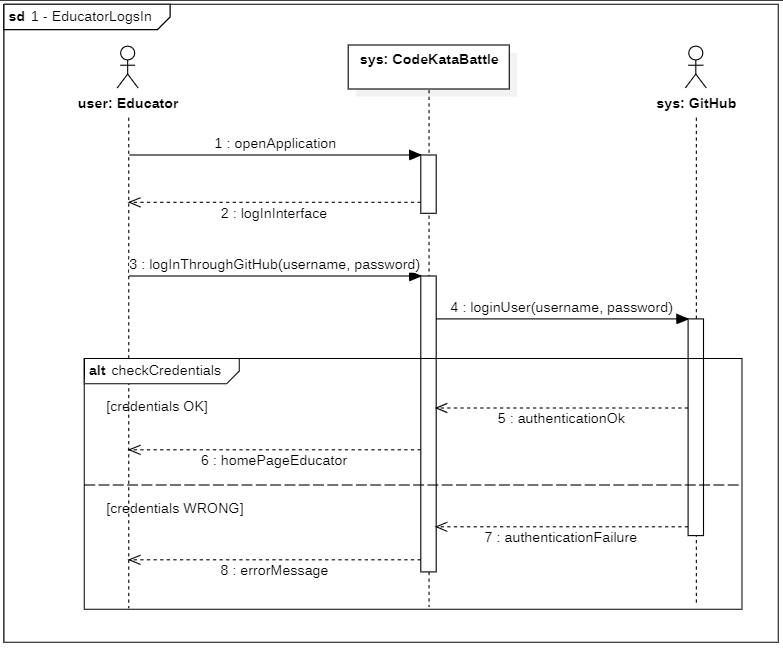
\includegraphics{1EducatorLogsIn}
\end{center}
\end{minipage}

\begin{minipage}{\textwidth}
\textbf{2 - StudentLogsIn}
\begin{center}
	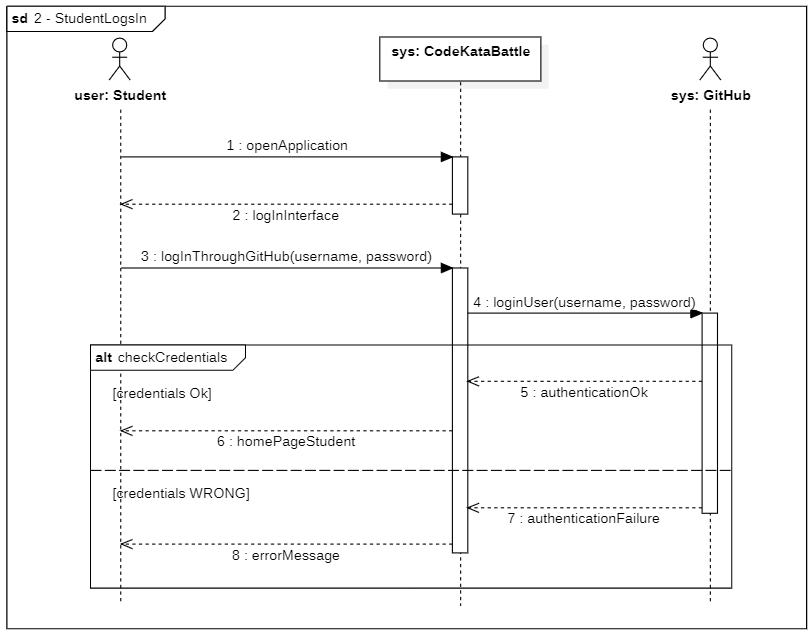
\includegraphics{2StudentLogsIn}
\end{center}
\end{minipage}

\begin{minipage}{\textwidth}
	\textbf{3 - CreateTournament}
	\begin{center}
		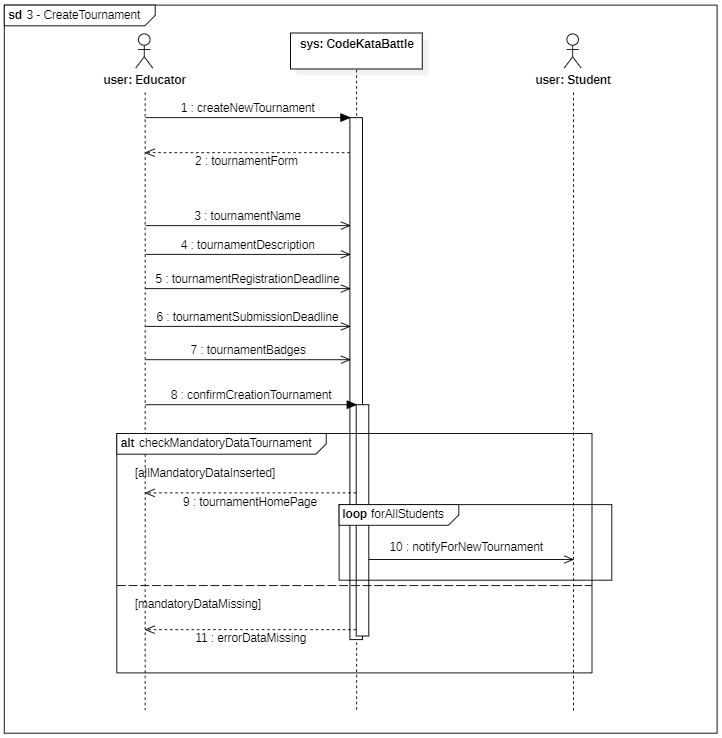
\includegraphics{3CreateTournament}
	\end{center}
\end{minipage}

\begin{minipage}{\textwidth}
	\textbf{4 - CreateBattle}
	\begin{center}
		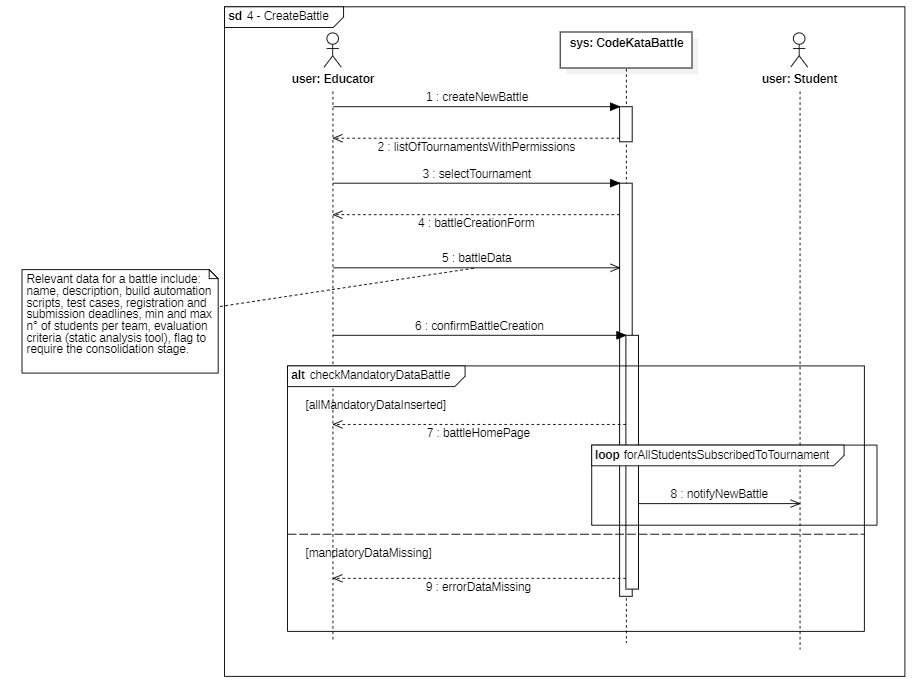
\includegraphics[scale=0.8]{4CreateBattle}
	\end{center}
\end{minipage}

\begin{minipage}{\textwidth}
	\textbf{5 - GrantPermissions}
	\begin{center}
		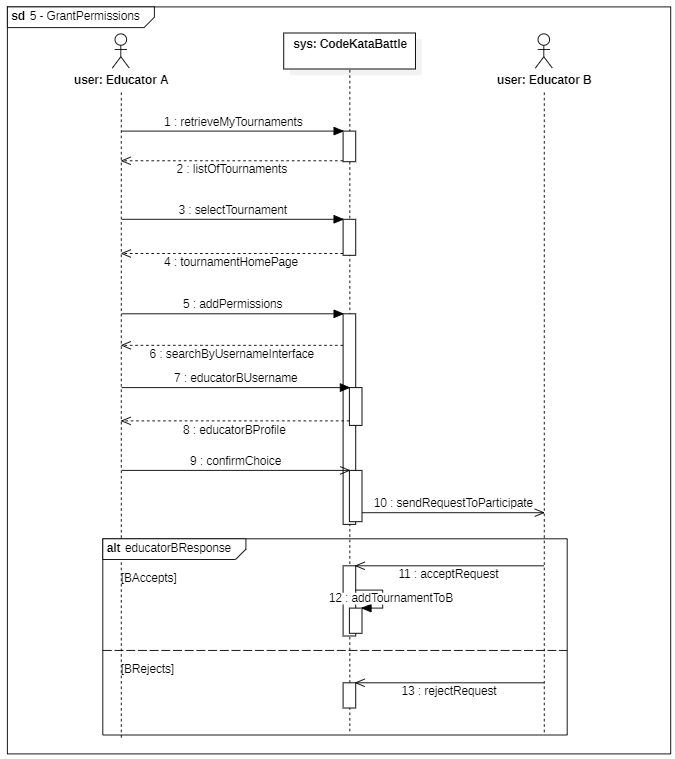
\includegraphics{5GrantPermissions}
	\end{center}
\end{minipage}

\begin{minipage}{\textwidth}
	\textbf{6 - SubscribeToTournament}
	\begin{center}
		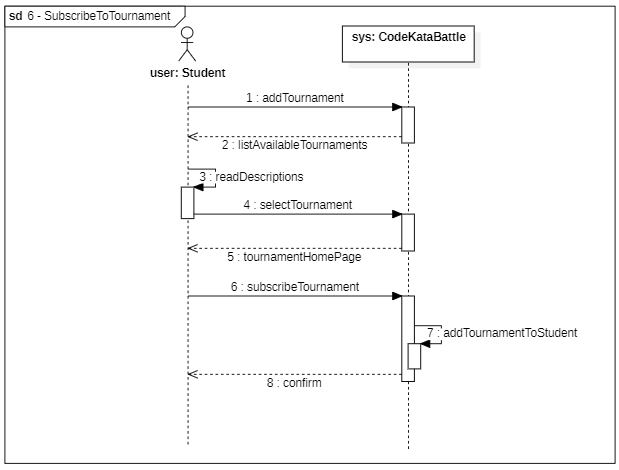
\includegraphics{6SubscribeToTournament}
	\end{center}
\end{minipage}

\begin{minipage}{\textwidth}
	\textbf{7 - JoinBattleAlone}
	\begin{center}
		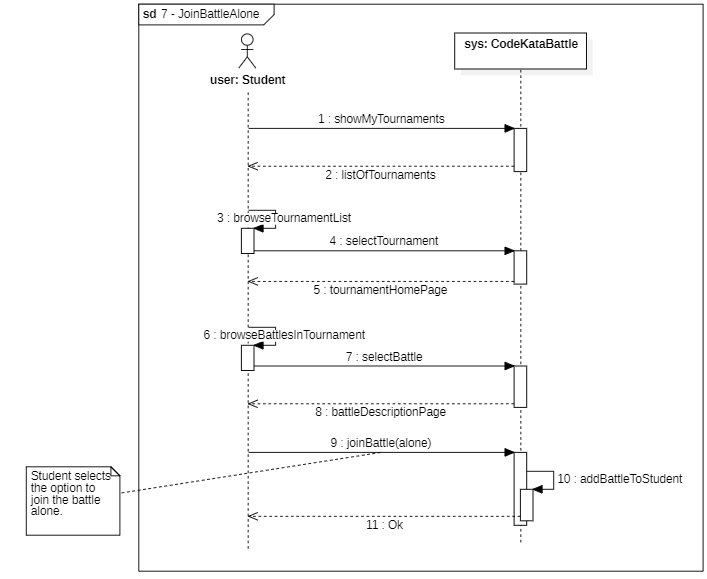
\includegraphics{7JoinBattleAlone}
	\end{center}
\end{minipage}

\begin{minipage}{\textwidth}
	\textbf{8 - JoinBattleAsTeam}
	\begin{center}
		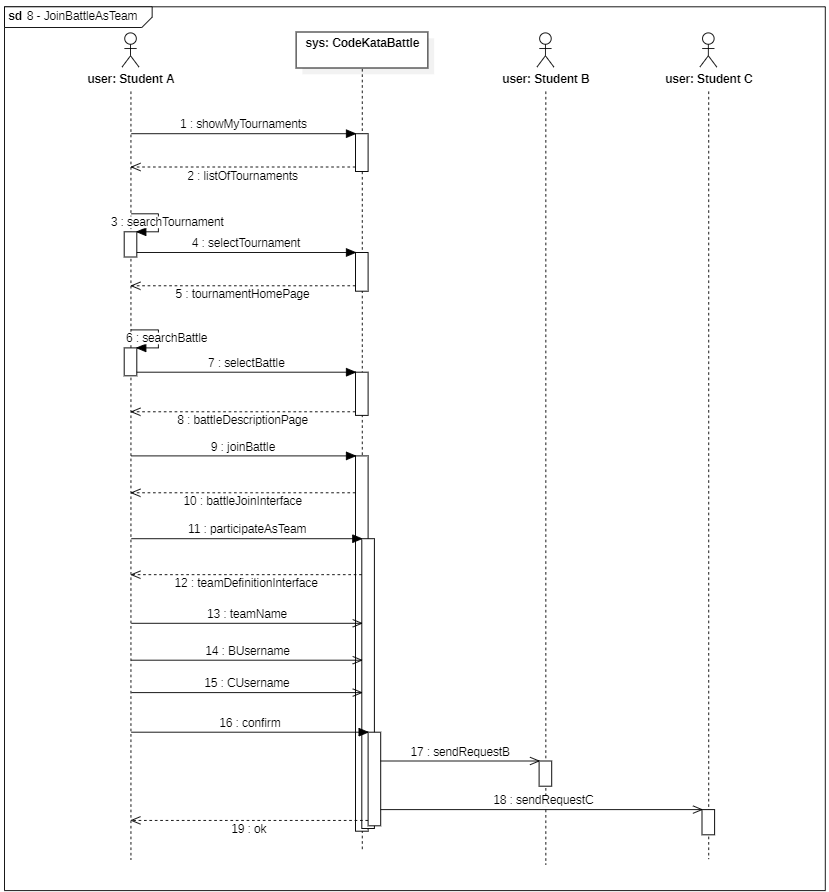
\includegraphics{8JoinBattleAsTeam}
	\end{center}
\end{minipage}

\begin{minipage}{\textwidth}
	\textbf{9 - CreateGitHubRepository}
	\begin{center}
		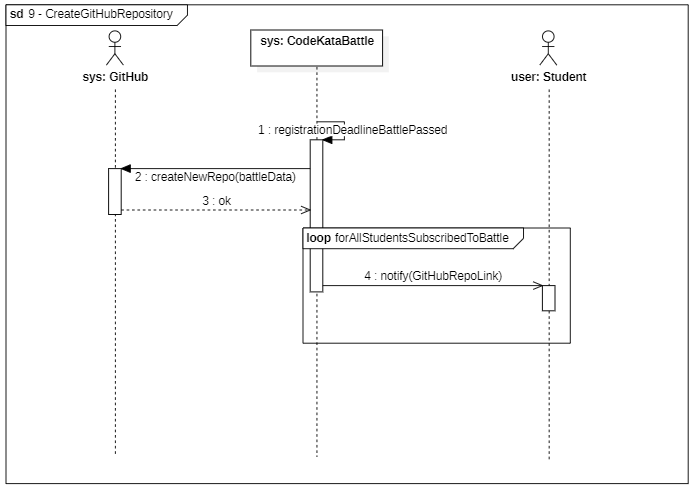
\includegraphics{9CreateGitHubRepository}
	\end{center}
\end{minipage}

\begin{minipage}{\textwidth}
	\textbf{10 - PushSolutionGitHub}
	\begin{center}
		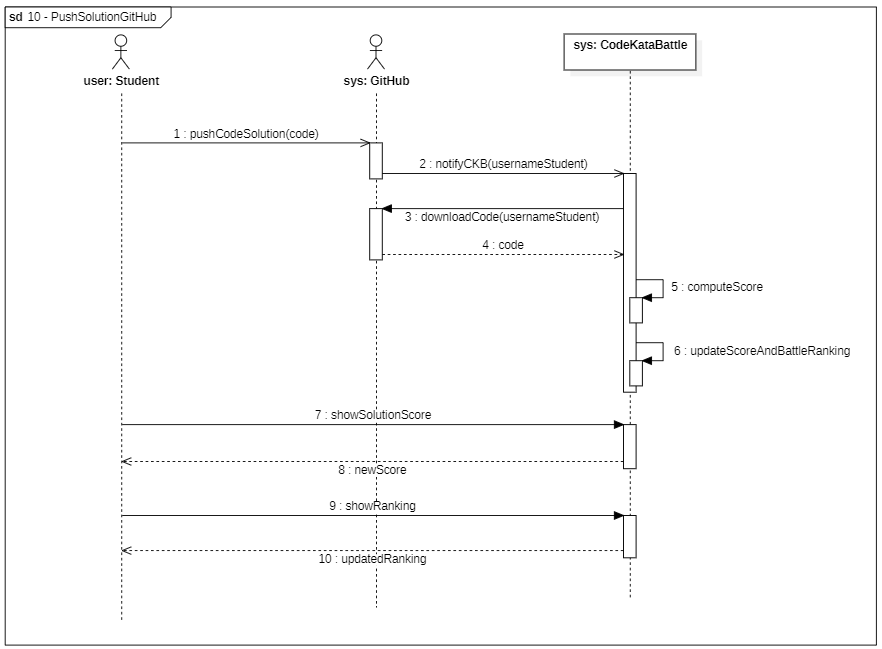
\includegraphics[scale=0.8]{10PushSolutionGitHub}
	\end{center}
\end{minipage}

\begin{minipage}{\textwidth}
	\textbf{11 - CalculateScore}
	\begin{center}
		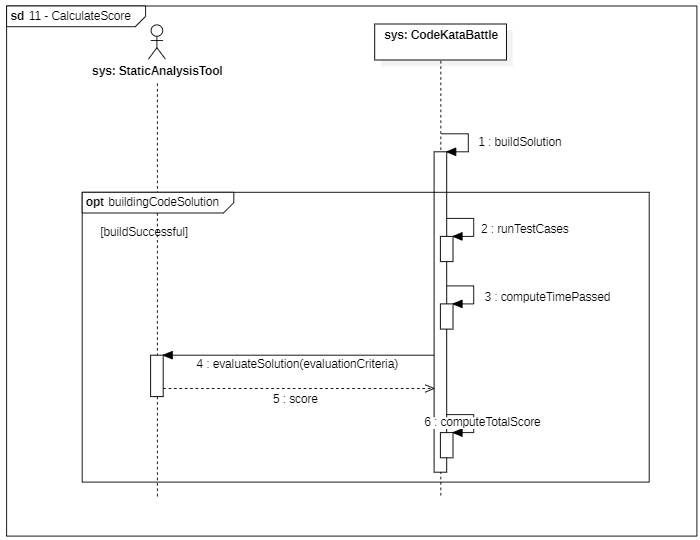
\includegraphics{11CalculateScore}
	\end{center}
\end{minipage}

\begin{minipage}{\textwidth}
	\textbf{12 - EvaluateSolutions}
	\begin{center}
		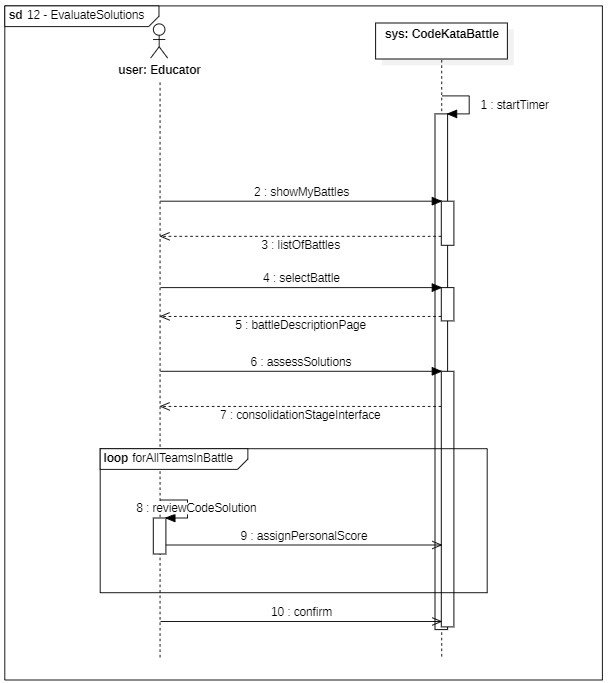
\includegraphics{12EvaluateSolutions}
	\end{center}
\end{minipage}

\begin{minipage}{\textwidth}
	\textbf{13 - TerminateBattle}
	\begin{center}
		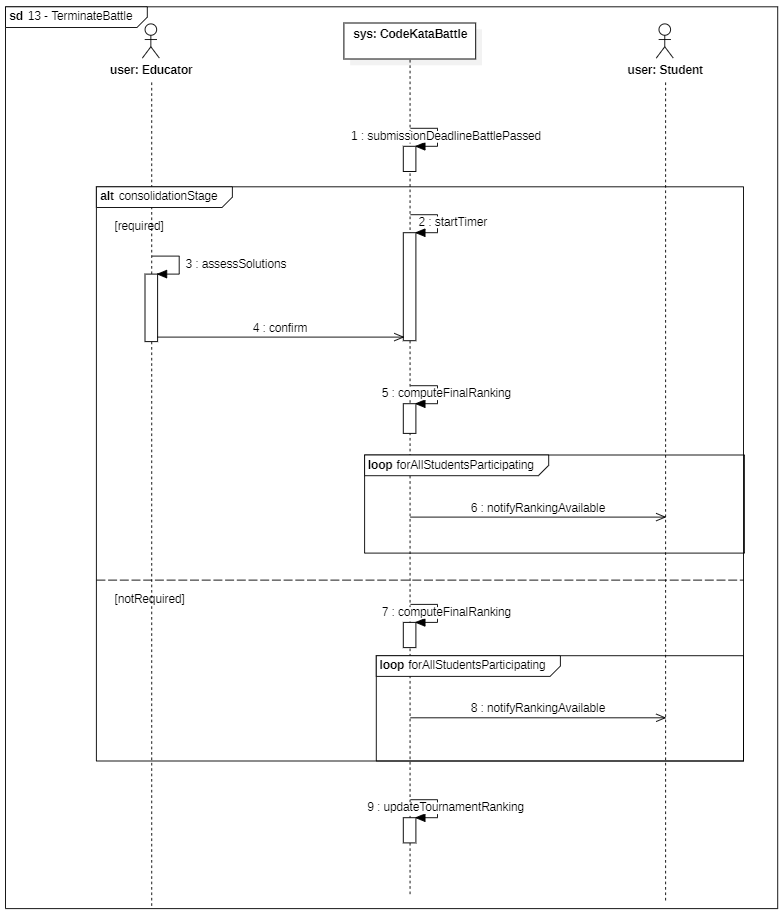
\includegraphics{13TerminateBattle}
	\end{center}
\end{minipage}

\begin{minipage}{\textwidth}
	\textbf{14 - CloseTournament}
	\begin{center}
		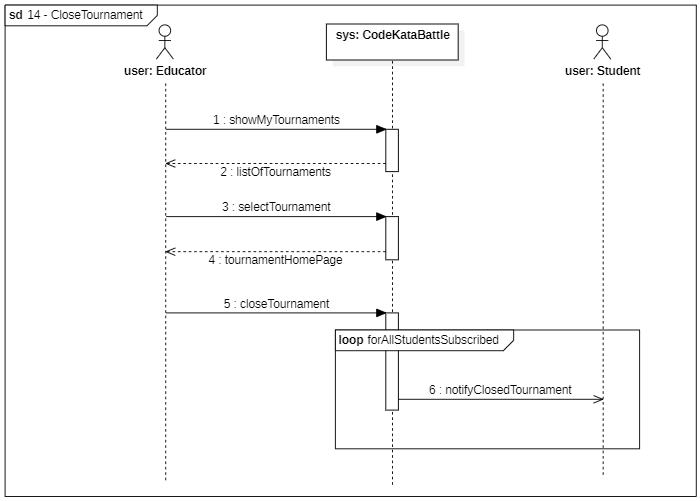
\includegraphics{14CloseTournament}
	\end{center}
\end{minipage}

\begin{minipage}{\textwidth}
	\textbf{15 - OpenTournamentRanking}
	\begin{center}
		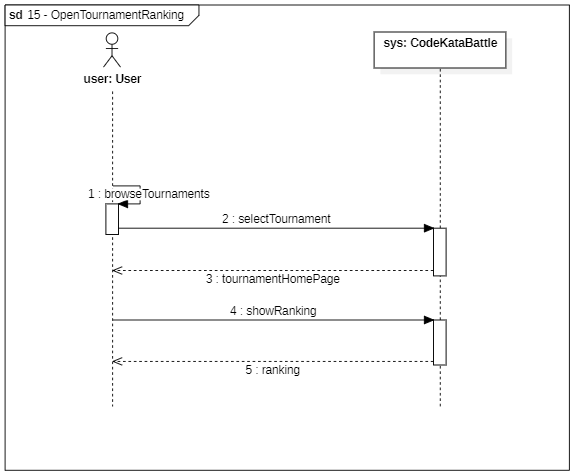
\includegraphics{15OpenTournamentRanking}
	\end{center}
\end{minipage}

\begin{minipage}{\textwidth}
	\textbf{16 - OpenBattleRanking}
	\begin{center}
		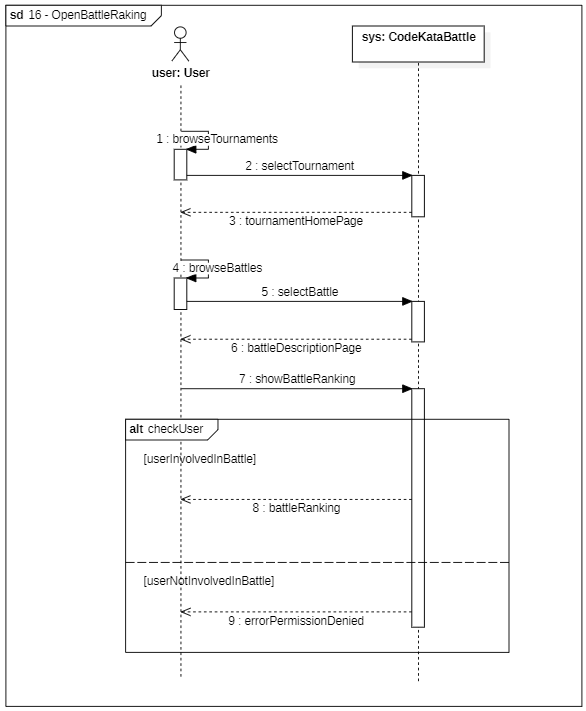
\includegraphics{16OpenBattleRanking}
	\end{center}
\end{minipage}

\begin{minipage}{\textwidth}
	\textbf{17 - ShowProfileAndBadges}
	\begin{center}
		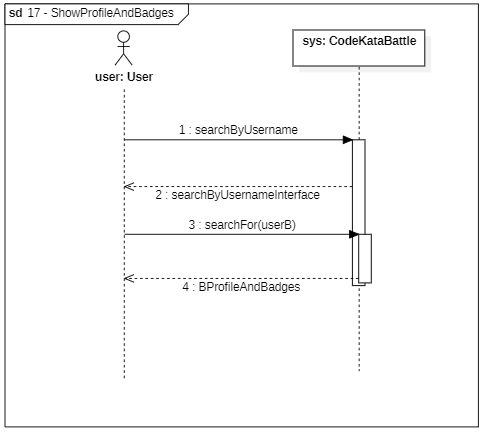
\includegraphics{17ShowProfileAndBadges}
	\end{center}
\end{minipage}
\subsubsection{Requirements Mapping}

\hspace{0.5cm}

\begin{tabular}{|p{8cm}|p{8cm}|}
\hline
\multicolumn{2}{|p{16cm}|}{[G1] The system allows students to practice and improve their coding skills by developing solutions to code kata battles.}\\
\hline
 & Qui\\
Ciaoooooooooo & ciaooooo \\
\hline
\end{tabular}

\vspace{1cm}

\begin{tabular}{|p{8cm}|p{8cm}|}
\hline
\multicolumn{2}{|p{16cm}|}{[G2] The system provides to educators a platform to publish code kata battles and easily manage tournaments and battles for students.}\\
\hline
Plutooooooooooo & Qui\\
Ciaoooooooooo & ciaooooo \\
\hline
\end{tabular}

\vspace{1cm}

\begin{tabular}{|p{8cm}|p{8cm}|}
\hline
\multicolumn{2}{|p{16cm}|}{[G3] The system makes the task of coding battles' solutions as fun as possible, introducing elements like competitiveness, rankings, teamwork and badges (or rewards).}\\
\hline
Plutooooooooooo & Qui\\
Ciaoooooooooo & ciaooooo \\
\hline
\end{tabular}
\newpage
\subsection{Performance Requirements}
The \textit{Code Battle} application must deliver efficient performance to meet the demands of students and educators engaging in coding challenges. The system should aim for low latency, ensuring that the time between user interactions and system responses does not exceed a few seconds under normal internet conditions, but it not a strict condition due to the nature of the application. It is acknowledged that users with slower internet connections may experience increased response times due to external factors beyond the system's control. The application should include mechanisms to detect and handle such situations effectively, but it is not mandatory. 


\subsection{Design Constraints}
\subsubsection{Standard Compliance}
In accordance with data privacy standards, the \app application operates within the framework of the General Data Protection Regulation (GDPR) in order to guarantee the privacy for students and educators data. This regulation governs data protection and privacy for individuals within the European Union (EU) and 
the European Economic Area (EEA). 
The application also adopts international standards for date and time representation.


\subsubsection{Hardware Limitations}
Students and educators hardware requirements are:
\begin{itemize}
    \item Internet connection (2G/3G/4G/5G/Wi-Fi)
    \item iOS/Android smartphone or computer with any modern web browser installed (Chrome, Opera, Firefox, Edge, and others)
\end{itemize}

\subsubsection{Other Constraints}
\newpage
\subsection{Software System Attributes}
\subsubsection{Reliability}
\subsubsection{Availability}
Given that \textit{Code Battle} is not an emergency service, the system can maintain an availability rate less then 99.9 percent. The average time between a fault occurrence and service recovery (MTTR) should be contained at a maximum of 7 days out of 365 per year. This implies that the service could remain highly available still not being completely reliable.


\subsubsection{Security}
As the system stores sensitive personal information about students and educators, security is of great importance. The central database must be fortified with comprehensive security measures to prevent external and internal attacks. Passwords stored in the data store must be encrypted, and in the case of password recovery, clear-text transmission should be avoided. All the channel of communication (e.g. notifications, mails) are assured to be encrypted in relation to the information contained in their messages (e.g. a password recovery is different from a reminder notification). Communication over the internet must utilize encryption to prevent traffic sniffing and spoofing, ensuring privacy and data consistency. 


\subsubsection{Maintainability}
\subsubsection{Portability}
The application must be developed as a web application, so it can be used by smartphones, tablets and computers having modern web browser. In other words, the web application should be compatible with any operating system (e.g., Windows, Mac OS, Linux) that supports a web browser. For this reason it could be developed in a common programming language which guarantees the use of a virtual machine employed in the market (e.g. C, C++, C\# don't seem to be a good choice; instead Java or Python do) 


\newpage
\clearpage
\section{Alloy}
\lstset{
  language=alloy,
  basicstyle=\small\ttfamily,
  breaklines=true,
  showstringspaces=false
}
In this section it is provided a representation of the world of CKB using the Alloy language. Every run and every check are commented in order to guarantee a syntactical correct compilation of the code: it is up to the reader to decide what to uncomment based on their will.

\lstinputlisting{4Alloy/res/third_model.als}

\subsection{Generated World}
\begin{figure}[h]
  \centering
  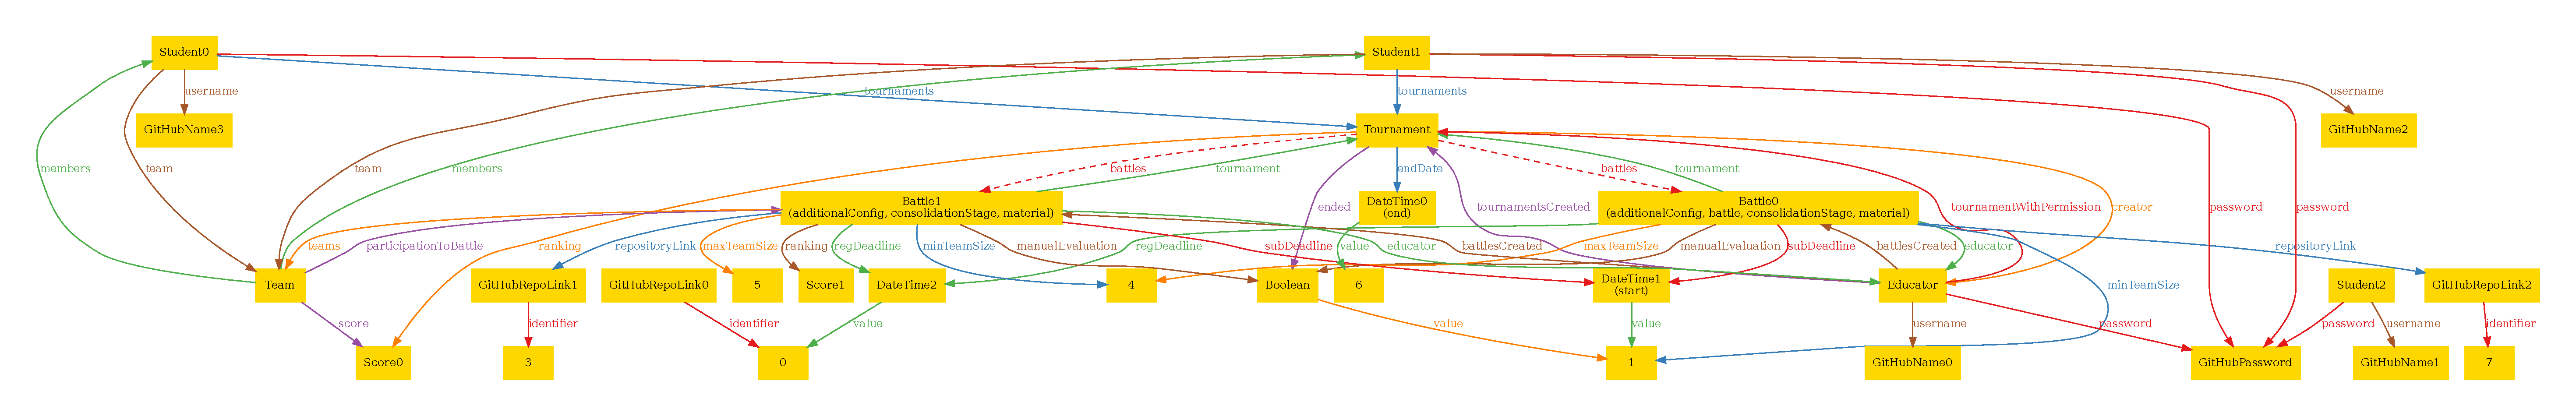
\includegraphics[width=1.1\linewidth]{4Alloy/res/general.pdf}
  \caption{The world generated by running \textit{general} predicate projected over nine signatures (ABS, CodeTest, ConsolidationStage, Description, EducatorMaterial, EvaluationCriteria, Macrovariables, Notification, String) in order to be more comprehensible. This world represents a normal situation of the model}
\end{figure}

\begin{figure}[h]
  \centering
  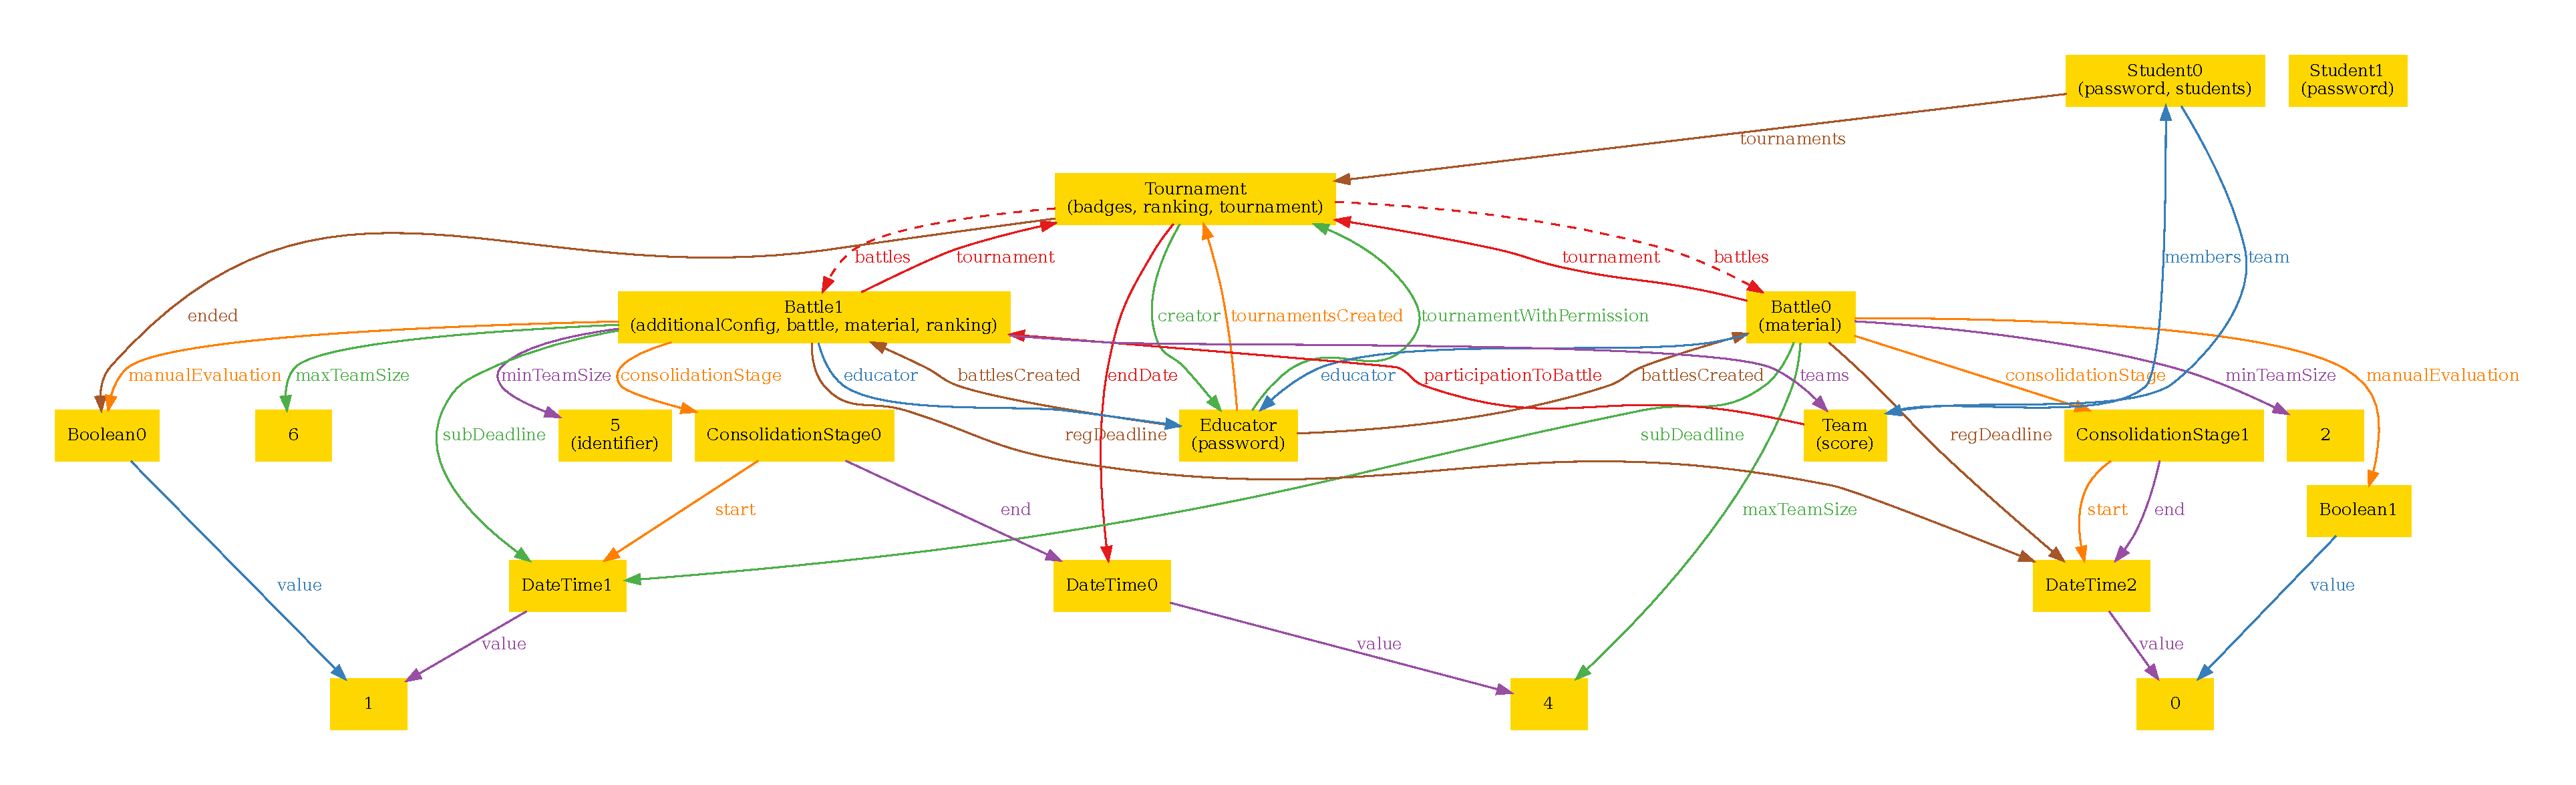
\includegraphics[width=1.1\linewidth]{4Alloy/res/noManualEvaluation.pdf}
  \caption{The world generated by running \textit{noManualEvaluation} predicate projected over thirteen signatures (ABS, Badge, CodeTest, Description, EducatorMaterial, EvaluationCriteria, GitHubName, GitHubPassword, GitHubRepoLink, Macrovariables, Notification, Score, String) in order to be more comprehensible. This world represents the situation where there is no manual evaluation for one battle out of two. It is useful in order to see the right aim of the model. Indeed, as you can see, in the case the manualEvaluation is not required (the boolean value equals 0) there is no consolidation stage, and viceversa}
\end{figure}

\afterpage{
  \clearpage
  \begin{figure}[h]
  \centering
  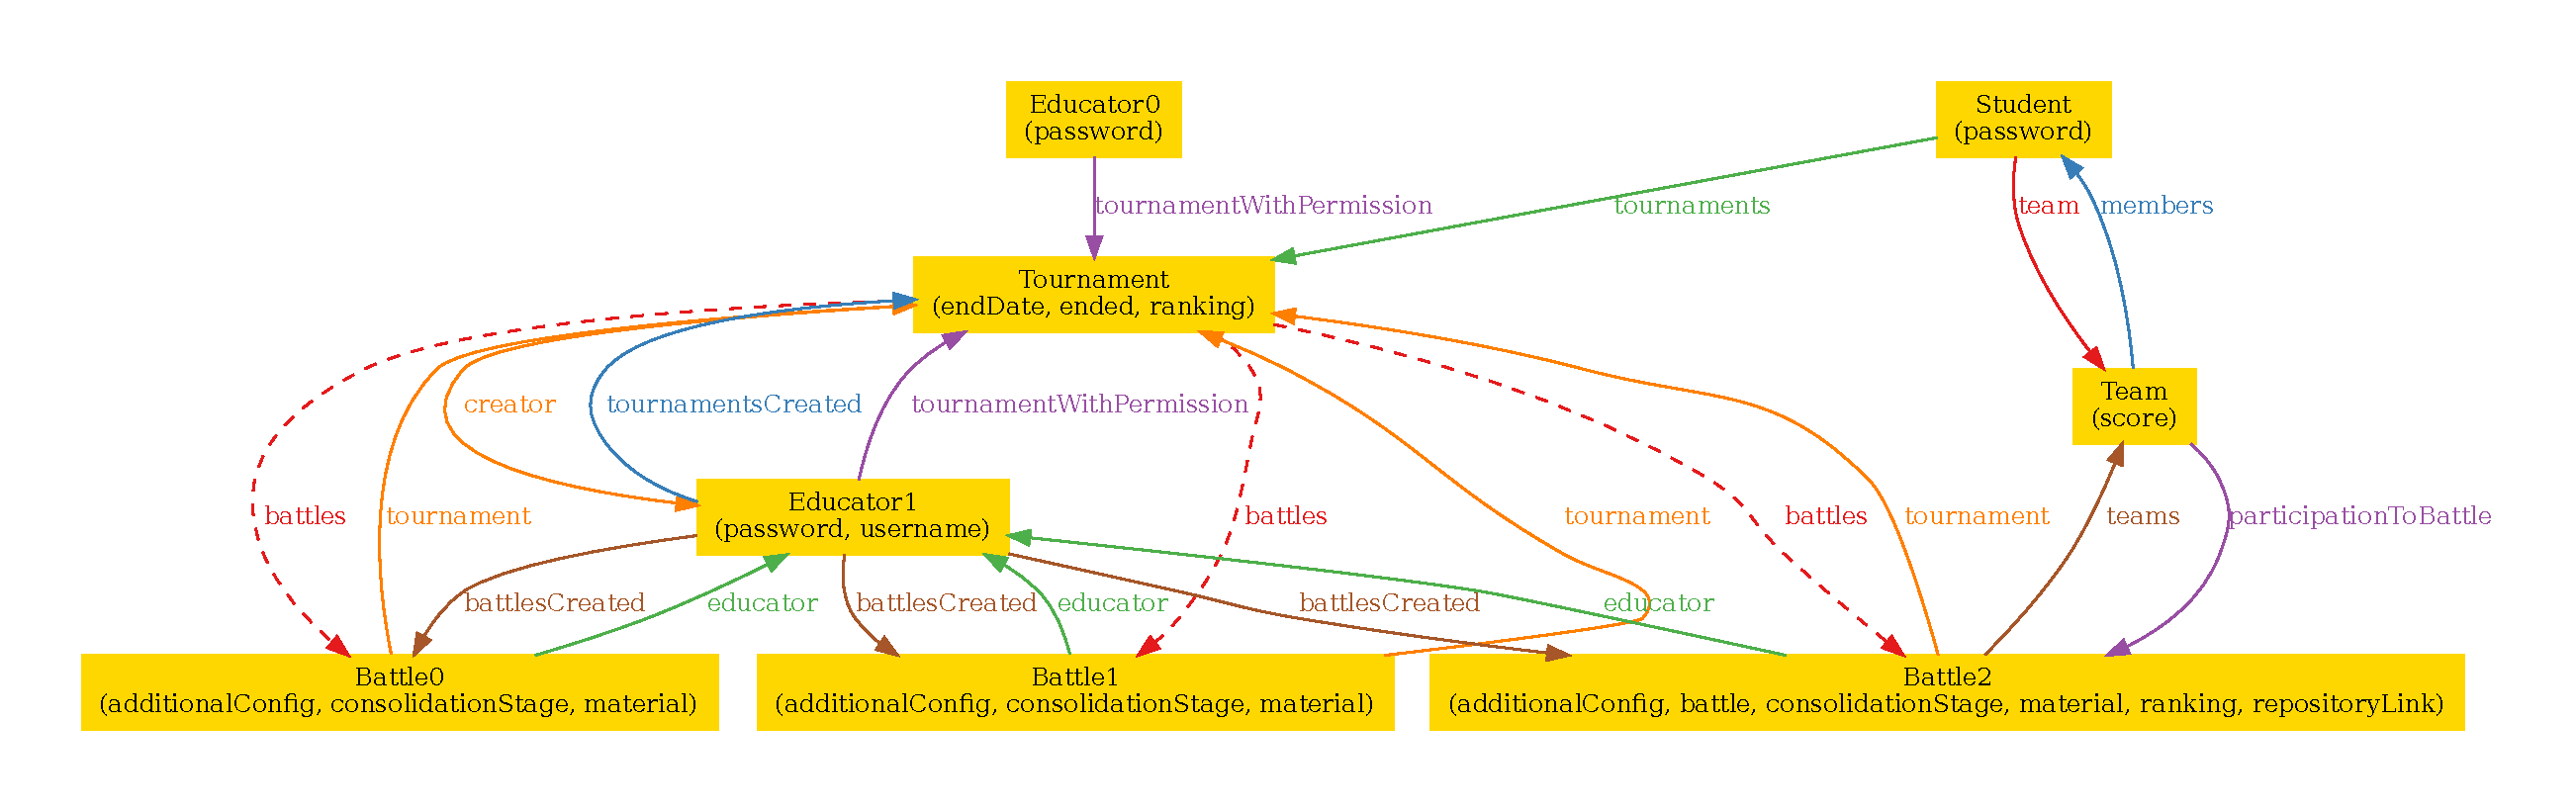
\includegraphics[angle=90, width=0.3\textwidth, height=1.35\textwidth]{4Alloy/res/educatorsWithOnlyPermission.pdf}
  \label{fig:educatorsWithOnlyPermission_alloy}
  \newpage
  \end{figure}
  \clearpage 
  \captionof{figure}{The world generated by running \textit{educatorsWithOnlyPermission} projected over seventeen signatures (ABS, Badge, Boolean, CodeTest, ConsolidationStage, DateTime, Description, EducatorMaterial, EvaluationCriteria, GitHubName, GitHubPassword, GitHubRepoLink, Int, Macrovariables, Notification, Score, String) in order to be more comprehensible. This world represents the situation where there are educator with permissions for a tournament they haven't created. As you can see, it cannot exist a tournament without a creator, but some educators can have tournaments with only the permission, without having created them}
}




\clearpage




\section{Effort spent}
\begin{table}[h]
  \centering
  \begin{tabular}{|p{1.5cm}|p{1.5cm}|p{1.5cm}|p{1.5cm}|p{1.5cm}|}
    \hline
     Studente & Introduction & Overall Description & Specific Requirements & Alloy \\
    \hline
    Alessandro & 5 & 12 & 15 & 30 \\
    \hline
    Matteo & 17 & 12 & 9 & Cell 4 \\
    \hline
    Sara & 0 & 15 & 5 & 0 \\
    \hline
  \end{tabular}
  \caption{Time spent on every section of the RASD for each student}
  \label{tab:effort}
\end{table}

\section{References}
%\bibliographystyle{apalike}
%\bibliography{example}

\end{document}
